\documentclass[11pt,a4paper]{article}

\usepackage[margin=1in]{geometry}
\usepackage{amsmath,amssymb}
\usepackage{booktabs}
\usepackage{graphicx}
\usepackage{subcaption}
\usepackage{array}
\usepackage{xcolor}
\usepackage{hyperref}
\usepackage{placeins}
\usepackage{enumitem}

\hypersetup{colorlinks=true,linkcolor=black,urlcolor=blue,citecolor=black}
\setlength{\parindent}{0pt}
\setlength{\parskip}{0.45em}
\setlist[itemize]{leftmargin=1.5em,itemsep=0.15em,topsep=0.2em}

\newcommand{\draftnote}[1]{\textcolor{gray}{\emph{#1}}}
\newenvironment{reporthint}{%
  \begin{quote}
  \begingroup\color{gray}\small
  \textbf{What to report.}
  \begin{itemize}
}{%
  \end{itemize}
  \endgroup
  \end{quote}
}
\newcommand{\twodpoint}{(x,y)}
\newcommand{\threedpoint}{(x,y,z)}

\newcommand{\figslot}[4]{%
  \begin{figure}[htbp]
    \centering
    \IfFileExists{#2}{%
      \includegraphics[width=0.86\linewidth]{#2}%
    }{%
      \fbox{%
        \begin{minipage}[c][0.22\textheight][c]{0.82\linewidth}
          \centering
          \textbf{Insert figure}\\[0.5em]
          \texttt{\detokenize{#2}}\\[0.5em]
          \draftnote{#3}
        \end{minipage}%
      }%
    }
    \caption{#4}
    \label{#1}
  \end{figure}
}

\newcommand{\smallmatrixslot}[1]{%
  \[
    #1 =
    \begin{pmatrix}
      \cdots & \cdots & \cdots\\
      \cdots & \cdots & \cdots\\
      \cdots & \cdots & \cdots
    \end{pmatrix}
  \]
}

\title{7.3 Minimisation Methods}

\begin{document}
\maketitle

\section*{Question 1: Shape and Analytic Minima}

\begin{figure}[htbp]
\centering
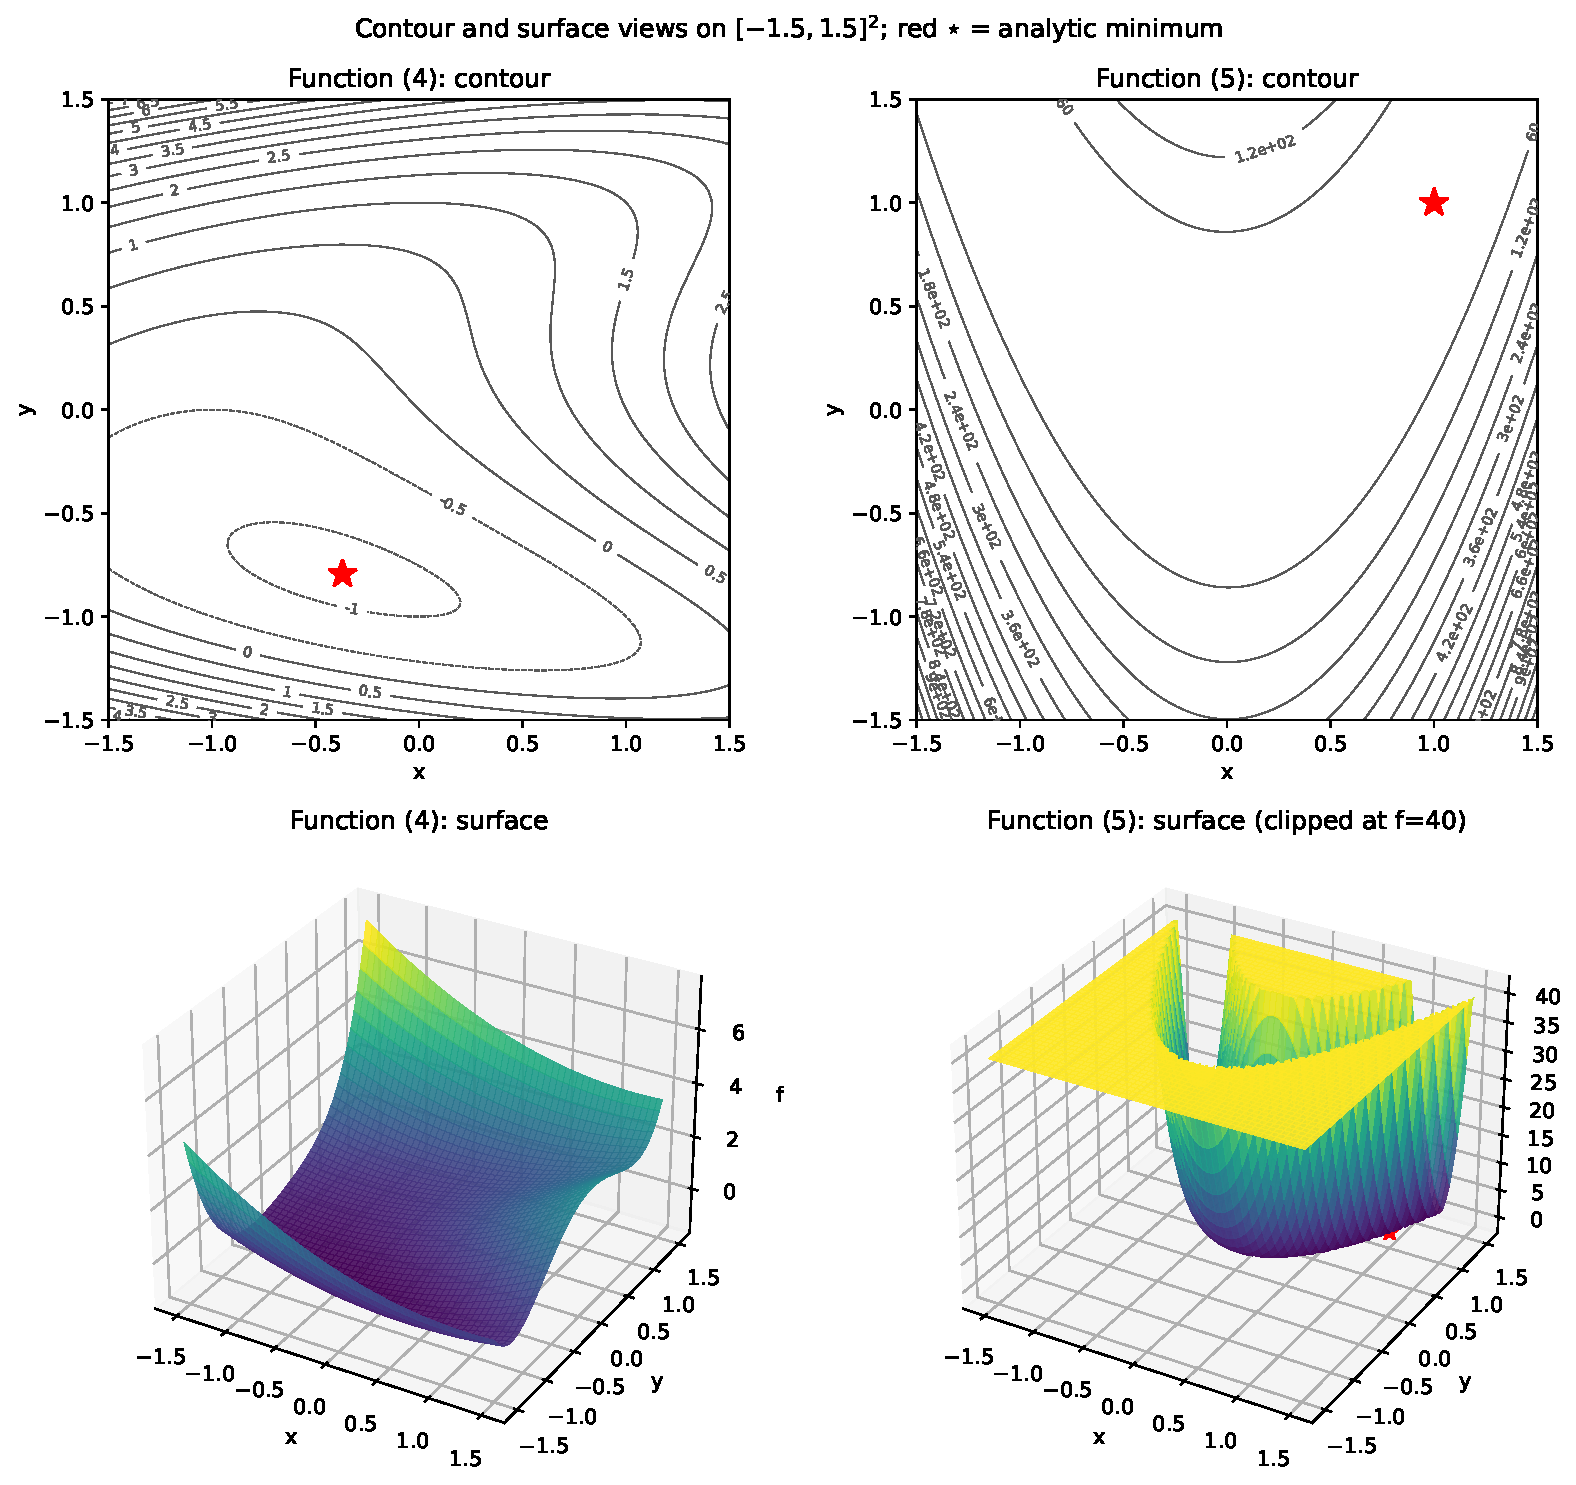
\includegraphics[width=0.95\linewidth]{figures/q1_contours.pdf}
\caption{Contour and surface plots of functions (4) and (5) on
\([-1.5,1.5]^{2}\); red stars mark the analytic minima.}
\label{fig:q1-contours}
\end{figure}

\begin{table}[htbp]
\centering
\caption{Analytic minima of the two two-variable objectives.}
\label{tab:q1-minima}
\begin{tabular}{lll}
\toprule
Function & Minimiser \((x^{*},y^{*})\) & \(f^{*}\)\\
\midrule
(4) & \((-0.3700,\,-0.7937)\) & \(-1.0953\)\\
(5) & \((1,\,1)\) & \(0\)\\
\bottomrule
\end{tabular}
\end{table}

\textbf{Function (4).}
Solving \(\partial_x f = 1+x-y^{2} = 0\) for \(x = y^{2}-1\) and substituting into \(\partial_y f = 1-2y+4y(y^{2}-x/2) = 0\) gives \(1+2y^{3}=0\). Since \(y\mapsto 2y^{3}\) is strictly increasing on \(\mathbb{R}\), the equation has the unique real root \(y^{*} = -2^{-1/3}\), so \(x^{*} = 2^{-2/3}-1\). The Hessian at \((x^{*},y^{*})\) is \(H = \bigl(\begin{smallmatrix}1 & 2^{2/3}\\ 2^{2/3} & 10\cdot 2^{-2/3}\end{smallmatrix}\bigr)\) with \(\det H = 6\cdot 2^{-2/3} = 3\cdot 2^{1/3}\approx 3.78 > 0\) and \(\operatorname{tr} H > 0\); by the second-derivative test, \((x^{*},y^{*})\) is a local minimum. Coercivity: in polar coordinates the quartic \((y^{2}-x/2)^{2}\) has leading term \(r^{4}\sin^{4}\theta\), which dominates for \(\sin\theta\ne 0\); along \(\sin\theta=0\) (i.e.\ \(y=0\)), \(f = x^{2}/4 + x\to\infty\) as \(|x|\to\infty\). Hence the unique stationary point is the global minimum. Eliminating \(x=y^{2}-1\) reduces \(f\) to \(g(y) = -\tfrac12 + y + y^{4}/2\), giving \(f^{*} = g(y^{*}) = -\tfrac{1}{2} - 2^{-1/3} + 2^{-7/3} \approx -1.0953\).

\textbf{Function (5).}
$\forall x,y \in \mathbb{R}$, $f = (1-x)^{2} + 80(y-x^{2})^{2} \ge 0$ with equality iff $y = x^{2}$ and $x = 1$. This corresponds to $(x^{*},y^{*}) = (1,1)$ and $f^{*} = 0$, making it a unique global minimum.\FloatBarrier

\section*{Questions 2--3: Steepest Descents}

% Include enough output to show the program worked: iteration path plot, values of
% lambda*, f(x_n), and decreases. Use comments to interpret the results rather than
% merely repeating table entries.

\subsection*{Question 2: Function (4)}

\begin{figure}[htbp]
\centering
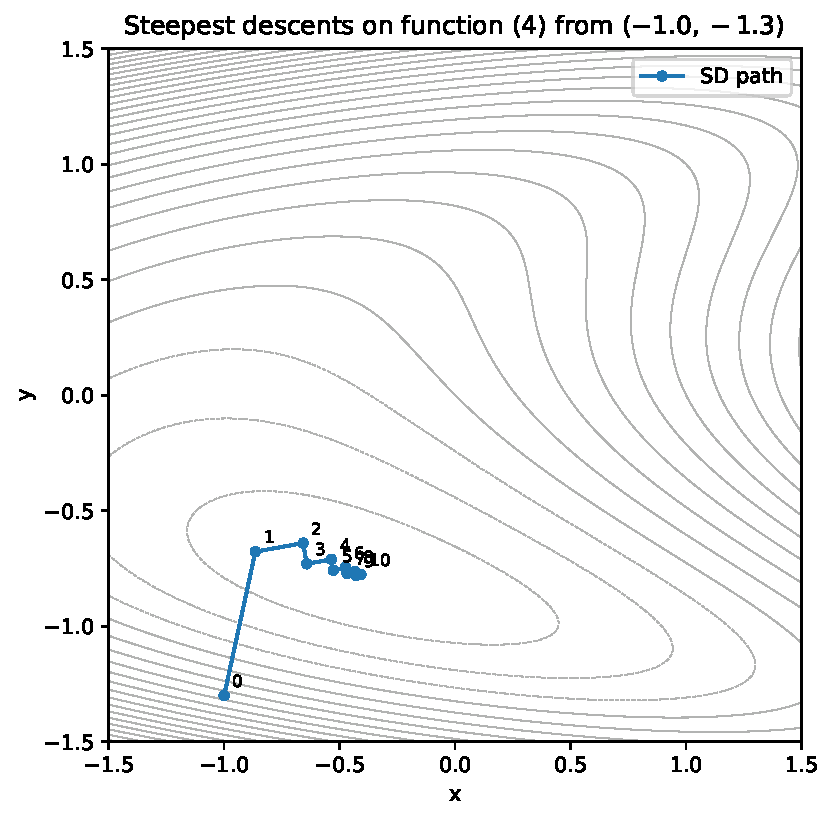
\includegraphics[width=0.72\linewidth]{figures/q2_steepest_function4_path.pdf}
\caption{Steepest-descents path on function (4) from \((-1.0,-1.3)\); ten iterations, numbered, with contours of \(f\) for reference.}
\label{fig:q2-path}
\end{figure}

\begin{table}[htbp]
\centering
\caption{Steepest-descents trace for function (4) from \((-1.0,-1.3)\). Line search: grid search on \(\lambda\in[0,2]\) with \(\Delta\lambda=10^{-4}\) (20001 points), giving \(\lambda^{\ast}\) to four decimals.}
\label{tab:q2-trace}
\begin{tabular}{rrrrrr}
\toprule
\(n\) & \(x_n\) & \(y_n\) & \(\lambda_n^\ast\) & \(f(x_n)\) & \(\Delta f_n\)\\
\midrule
0  & \(-1.0000\) & \(-1.3000\) & --      & \(+1.0561\)   & --\\
1  & \(-0.8599\) & \(-0.6544\) & 0.0829  & \(-1.02119\)  & \(-2.077\)\\
2  & \(-0.3839\) & \(-0.7577\) & 1.652   & \(-1.09201\)  & \(-7.08\times 10^{-2}\)\\
3  & \(-0.3905\) & \(-0.7881\) & 0.1572  & \(-1.09515\)  & \(-3.14\times 10^{-3}\)\\
4  & \(-0.3705\) & \(-0.7924\) & 1.714   & \(-1.09527\)  & \(-1.22\times 10^{-4}\)\\
5  & \(-0.3707\) & \(-0.7935\) & 0.1492  & \(-1.09528\)  & \(-4.20\times 10^{-6}\)\\
6  & \(-0.3701\) & \(-0.7937\) & 1.706   & \(-1.09528\)  & \(-1.43\times 10^{-7}\)\\
7  & \(-0.3701\) & \(-0.7937\) & 0.1490  & \(-1.09528\)  & \(-5.66\times 10^{-9}\)\\
8  & \(-0.3700\) & \(-0.7937\) & 1.697   & \(-1.09528\)  & \(-2.23\times 10^{-10}\)\\
9  & \(-0.3700\) & \(-0.7937\) & 0.1493  & \(-1.09528\)  & \(-9.84\times 10^{-12}\)\\
10 & \(-0.3700\) & \(-0.7937\) & 1.598   & \(-1.09528\)  & \(-4.19\times 10^{-13}\)\\
\bottomrule
\end{tabular}
\end{table}

\textbf{Line-search quantisation.}
The 20001-point grid on \(\lambda\in[0,2]\) with \(\Delta\lambda=10^{-4}\) gives a per-step error bounded by \(\tfrac18\phi''(\lambda^{\ast})(\Delta\lambda)^{2}\lesssim 10^{-9}\), far below the observed \(|\Delta f_n|\) at every iteration except \(n=10\) where the two are comparable. Quantisation is therefore not the limiting error and will not be revisited.

\textbf{Linear tail and value estimate.}
On a convex quadratic, by the Kantorovich inequality~\cite{luenberger-ye}:
\[
f_{n+1}-f^{*} \;\le\; \left(\frac{\kappa-1}{\kappa+1}\right)^{\!2}\!(f_{n}-f^{*}), \qquad \kappa=\frac{\lambda_{\max}(H)}{\lambda_{\min}(H)},
\]
giving worst-case \(r_{K}=0.717\) at the Q1 Hessian \(\kappa\approx 12\) (\(\lambda_{\min}\approx 0.56,\,\lambda_{\max}\approx 6.74\)). The observed per-step ratios \(r_n=|\Delta f_{n+1}|/|\Delta f_n|\) from Table~\ref{tab:q2-trace}:
\[
\begin{array}{c|ccccccccc}
n & 1 & 2 & 3 & 4 & 5 & 6 & 7 & 8 & 9\\\hline
r_n & 0.034 & 0.044 & 0.039 & 0.034 & 0.034 & 0.040 & 0.039 & 0.044 & 0.043
\end{array}
\]
sit at \(r\approx 0.04\), an order of magnitude below the Kantorovich worst case. The mechanism: exact line search forces \(g_{n+1}\perp g_n\), and in 2-D the gradient returns to its original direction (up to scale) after two steps, producing the 2-cycle visible in Table~\ref{tab:q2-trace} as \(\lambda^{\ast}\) alternating between \(\sim 0.15\) and \(\sim 1.7\). The per-step contraction of this cycle depends on where \(g\) sits in the eigenbasis of \(H\); Kantorovich's bound is attained only at one specific orientation, and our iterate doesn't visit it. Coarser line-search noise would scramble the 2-cycle back toward typical-Kantorovich behaviour (\(r\approx 0.6\) with \(\Delta\lambda=10^{-2}\)), but \(\Delta\lambda=10^{-4}\) is precise enough to preserve the fast cycle. Modelling the tail as geometric, \(f_{n}-f^{\ast}\approx (r/(1-r))|\Delta f_{n}|\); substituting \(|\Delta f_{10}|=4.2\times 10^{-13}\) and \(r=0.04\) gives \(f_{10}-f^{\ast}\approx 1.8\times 10^{-14}\), at the floating-point floor. Hence
\[
\boxed{\;f^{\ast}=-1.09528\pm 10^{-13},\qquad\text{i.e.\ machine-precision agreement.}\;}
\]

\textbf{Coordinate estimates.}
With the iterate having reached \(|g_{10}|=6.86\times 10^{-7}\), the Taylor expansion \(g(x^{\ast}+\varepsilon)=H\varepsilon+O(|\varepsilon|^{2})\) and the Rayleigh-quotient bound \(\lambda_{\min}(H)|\varepsilon|\le|H\varepsilon|\) give a direct error estimate
\[
|\varepsilon|=\|x_{10}-x^{\ast}\|\;\le\;\frac{|g_{10}|}{\lambda_{\min}(H)}+O(|\varepsilon|^{2})\;\approx\;1.2\times 10^{-6}.
\]
The actual displacement, computed against the Q1 closed form, is \(\|x_{10}-x^{\ast}\|=1.7\times 10^{-7}\) --- inside the bound by a factor of \(\sim 7\), reflecting that the gradient is well-aligned with \(\lambda_{\max}\)-eigenvectors near the minimum (Q1 Hessian's larger eigenvalue \(6.74\) dominates). The \emph{coordinate-by-coordinate} extrapolation used at the coarse-grid Q2 budget (interleaved geometric subsequences in \(x_n\) or \(y_n\)) is no longer informative: \(x_n\) is not monotone (\(x_2=-0.384\), \(x_3=-0.391\), \(x_4=-0.371\)) because the fine-grid line search overshoots and corrects within each pair, so a single-sided bound from the trace alone is loose.

\textbf{Value precision vs point precision.}
After 10 iterations: \(f^{\ast}\) to \(\sim 13\) digits (\(\varepsilon_f\sim 10^{-13}\)); \((x^{\ast},y^{\ast})\) to \(\sim 7\) digits (\(|\varepsilon|\sim 10^{-7}\)). The relation \(\varepsilon_f\sim|\varepsilon|^{2}\) up to \(O(1)\) shows one digit of value precision is gained from a half-digit of point precision; both ends are now far below the line-search quantisation floor.

\textbf{Why.}
Since \(g(x^{\ast})=0\), Taylor expansion at \(x=x^{\ast}+\varepsilon\) gives \(f(x^{\ast}+\varepsilon)=f^{\ast}+\tfrac12\,\varepsilon^{T}\!H\,\varepsilon+O(|\varepsilon|^{3})\): the linear term vanishes. Applying the Rayleigh-quotient bounds \(\lambda_{\min}(H)|\varepsilon|^{2}\le\varepsilon^{T}\!H\,\varepsilon\le\lambda_{\max}(H)|\varepsilon|^{2}\) then yields
\[
\sqrt{\frac{2\,\varepsilon_f}{\lambda_{\max}(H)}} \;\lesssim\; |\varepsilon| \;\lesssim\; \sqrt{\frac{2\,\varepsilon_f}{\lambda_{\min}(H)}}\,.
\]
Substituting \(\varepsilon_f\sim 10^{-13}\) and the Q1 eigenvalues bounds \(|\varepsilon|\in[1.7\times 10^{-7},\,6.0\times 10^{-7}]\), consistent with the observed \(|\varepsilon|=1.7\times 10^{-7}\). The relation \(\varepsilon_f\sim|\varepsilon|^{2}\) is universal at smooth non-degenerate minima: \(f\) is flat to first order and curved to second, so location precision is the binding constraint at fixed iteration budget --- not line-search quantisation, not value conditioning.

\subsection*{Question 3: Function (5)}

\begin{figure}[htbp]
\centering
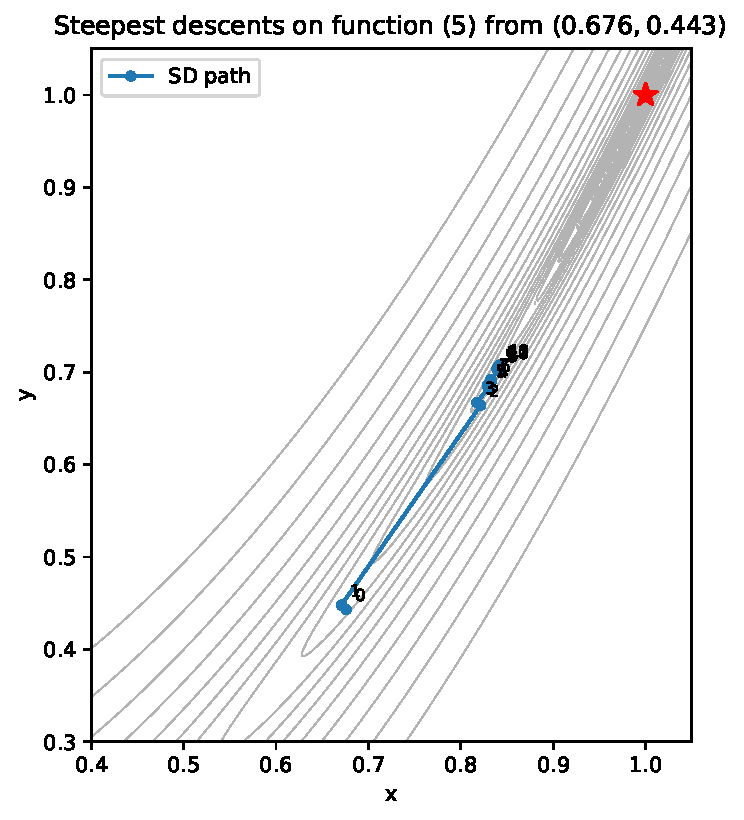
\includegraphics[width=0.70\linewidth]{figures/q3_steepest_function5_path.pdf}
\caption{Steepest-descents path on function (5) from $(0.676,0.443)$; twelve iterations, numbered, with contours of $f$ (log-spaced). Red $\star$ marks $(1,1)$. After step 1 the iterates cluster inside $[0.82,0.85]\times[0.66,0.71]$, crawling along the curved valley $y=x^{2}$.}
\label{fig:q3-path}
\end{figure}

\begin{table}[htbp]
\centering
\caption{Steepest-descents trace for function (5) from $(0.676,0.443)$. Same line search as Q2: grid on $\lambda\in[0,2]$ with $\Delta\lambda=10^{-4}$ (20001 points).}
\label{tab:q3-trace}
\begin{tabular}{rrrrrr}
\toprule
$n$ & $x_n$ & $y_n$ & $\lambda_n^\ast$ & $f(x_n)$ & $\Delta f_n$\\
\midrule
0  & $+0.6760$ & $+0.4430$ & --       & $+0.12060$ & --\\
1  & $+0.6708$ & $+0.4479$ & $0.0022$ & $+0.10872$ & $-1.19\times 10^{-2}$\\
2  & $+0.8215$ & $+0.6641$ & $0.6694$ & $+0.04104$ & $-6.77\times 10^{-2}$\\
3  & $+0.8173$ & $+0.6670$ & $0.0017$ & $+0.03345$ & $-7.59\times 10^{-3}$\\
4  & $+0.8307$ & $+0.6844$ & $0.1141$ & $+0.03128$ & $-2.17\times 10^{-3}$\\
5  & $+0.8287$ & $+0.6859$ & $0.0017$ & $+0.02940$ & $-1.88\times 10^{-3}$\\
6  & $+0.8334$ & $+0.6910$ & $0.0386$ & $+0.02876$ & $-6.35\times 10^{-4}$\\
7  & $+0.8324$ & $+0.6920$ & $0.0017$ & $+0.02816$ & $-6.09\times 10^{-4}$\\
8  & $+0.8405$ & $+0.7021$ & $0.0744$ & $+0.02701$ & $-1.15\times 10^{-3}$\\
9  & $+0.8391$ & $+0.7033$ & $0.0017$ & $+0.02595$ & $-1.06\times 10^{-3}$\\
10 & $+0.8416$ & $+0.7057$ & $0.0206$ & $+0.02564$ & $-3.04\times 10^{-4}$\\
11 & $+0.8409$ & $+0.7065$ & $0.0018$ & $+0.02534$ & $-2.98\times 10^{-4}$\\
12 & $+0.8427$ & $+0.7080$ & $0.0136$ & $+0.02514$ & $-2.04\times 10^{-4}$\\
\bottomrule
\end{tabular}
\end{table}

\textbf{Limit point.}
The unique stationary point of $f$ is $(1,1)$: $\partial_y f = 160(y-x^{2})=0\Rightarrow y=x^{2}$, then $\partial_x f = -2(1-x)=0\Rightarrow x=1$. The level set $\{f\le f_0\}$ is bounded, since $f\ge(1-x)^{2}$ gives $|x|\le 1+\sqrt{f_0}$ and $f\ge 80(y-x^{2})^{2}$ then bounds $|y|$. Hence $(x_n)$ is bounded; $f_n$ is monotone decreasing and bounded below by $0$, so $\Delta f_n\to 0$, and the standard SD bound $\Delta f_n\ge c|g_n|^{2}$ (for $c>0$ depending on local Hessian bounds) gives $|g_n|\to 0$. Every subsequential limit is therefore stationary, and uniqueness forces $x_n\to(1,1),\ f^{\ast}=0$.

\textbf{Linear tail and rate.}
$\lambda_n^{\ast}$ alternates: odd-$n$ steps have $\lambda_n^{\ast}\approx 0.002$ (iterate sits near $y=x^{2}$, $g_y\approx 0$, the short step along $-g_x$ is constrained by the curving floor); even-$n$ steps have $\lambda_n^{\ast}$ larger as the iterate drifts off-valley and $-g$ points back across. This is the zigzag across the narrow curved valley. Subsampling at even $n$ to remove zigzag noise:
\[
\begin{array}{c|ccccc}
n & 4 & 6 & 8 & 10 & 12\\\hline
f_n/f_{n-2} & 0.763 & 0.920 & 0.938 & 0.948 & 0.981
\end{array}
\]
$f_n/f_{n-2}$ is \emph{increasing} toward the two-step Kantorovich bound~\cite{luenberger-ye} $r_K^{2}=((\kappa-1)/(\kappa+1))^{4}\approx 1-8/\kappa$: at $(1,1)$, $H=\bigl(\begin{smallmatrix}642 & -320\\ -320 & 160\end{smallmatrix}\bigr)$ has eigenvalues $\approx 801.6,\,0.399$, $\kappa\approx 2.0\times 10^{3}$, $r_K\approx 0.998$; at the actual iterate $(x_{12},y_{12})=(0.843,0.708)$, direct calculation gives $\kappa\approx 0.85\times 10^{3}$, $r_K\approx 0.995$ (the small eigenvalue depends approximately linearly on $y-x^{2}$, so $\kappa$ varies between $\sim 10^{2}$ and $\sim 4\!\times\!10^{3}$ across the cluster). Using the late per-iteration rate $r\approx 0.99$ in $f_n-f^{\ast}\approx |\Delta f_n|/(1-r)$:
\[
f_{12}-f^{\ast}\approx 2\times 10^{-2},\qquad f^{\ast}\approx f_{12}-2\times 10^{-2}\approx 5\times 10^{-3}.
\]
This central estimate is uncertain because $\kappa$ (hence $r$) varies along the curved valley, so the fixed-$r$ geometric model is only a local surrogate. Combined with the analytic lower bound $f^{\ast}\ge 0$:
\[
\boxed{\;f^{\ast}\in[0,\,\sim\!10^{-2}]\;.}
\]

\textbf{Coordinate precision via the valley identity.}
Iterates lie approximately on $y=x^{2}$, so $f_n = (1-x_n)^{2}+80(y_n-x_n^{2})^{2}$ is dominated by the first term: at $n=12$, $(1-0.843)^{2}=0.0246\approx f_{12}=0.0251$ (the $2\%$ residual is the small $(y-x^{2})$ offset). Hence $|1-x_n|\approx\sqrt{f_n}$ gives a direct location estimate tighter than any interleaved-GP extrapolation: $|1-x_{12}|\approx 0.158$, so $x^{\ast}\in[0.84,1]$ and by the valley $y^{\ast}\in[0.71,1]$; 12 iterations have covered only $(1-0.158/0.324)\approx 51\%$ of the along-valley distance. The precision relation $\varepsilon_f\sim|\varepsilon|^{2}$ holds here in its \emph{along-valley} form with constant $1$ (not $\tfrac12\lambda_{\max}$), because $f(x,x^{2})=(1-x)^{2}$ has second derivative $2$.

\textbf{Sensitivity to $\lambda^{\ast}$.}

\begin{figure}[htbp]
\centering
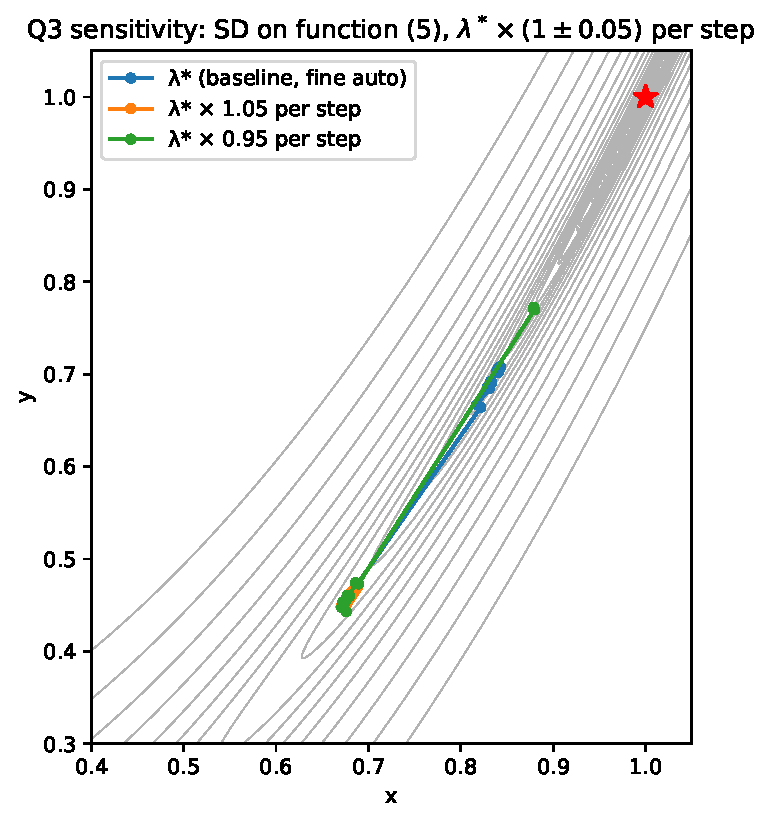
\includegraphics[width=0.72\linewidth]{figures/q3_steepest_function5_sensitivity.pdf}
\caption{SD on (5): baseline path and $\pm 5\%$ per-step perturbations of $\lambda^{\ast}$. Paths diverge from $n=2$, where the baseline step $\lambda_2^{\ast}=0.67$ amplifies any multiplicative perturbation directly into $|\Delta x|\sim 0.03$.}
\label{fig:q3-sens}
\end{figure}

Per-step $\pm 5\%$ perturbation gives final points: baseline $(0.843,0.708)$, $f=0.025$; $+5\%\to(0.688,0.470)$, $f=0.098$; $-5\%\to(0.879,0.772)$, $f=0.015$. The $+5\%$ run overshoots at the breakthrough step and climbs the opposite valley wall; the $-5\%$ run undershoots and stays on the near wall. Linearisation at exact line-search minimum: since $\phi'(\lambda^{\ast})=0$, a perturbation $\delta\lambda$ gives $\phi(\lambda^{\ast}+\delta\lambda)-\phi(\lambda^{\ast})=\tfrac12\phi''(\lambda^{\ast})\delta\lambda^{2}+O(\delta\lambda^{3})$, so the per-step \emph{$f$-value} error is $O(\delta\lambda^{2})$ on any smooth $f$. The per-step \emph{position} error, however, is $O(\delta\lambda)$: $\delta x_{n+1}=\delta\lambda_n s_n$, hence $\delta g_{n+1}\approx -\delta\lambda_n H g_n$, growing by $\|H\|\cdot\delta\lambda$. On a tight curved valley like (5), this $O(\delta\lambda)$ position drift is not absorbed because the next baseline step depends sensitively on the iterate's distance from the valley curve $y=x^{2}$; a $\delta\lambda$ kick translates into a different segment of the long valley, and over many steps the cumulative drift dominates. Line-search accuracy is therefore binding for path stability, though not for per-step value precision.

\textbf{Why SD is inefficient.}
Three reinforcing causes, each visible in Figure~\ref{fig:q3-path}:
\emph{(a) Anisotropy.} Along-valley curvature is $d^{2}/dx^{2}(1-x)^{2}=2$, cross-valley is $\partial^{2}f/\partial y^{2}=160$, giving an axis-aligned curvature ratio $\approx 80$. The Hessian's principal axes at $(1,1)$ are not aligned with $(x,y)$, so the spectral condition number is larger: $\kappa\approx 2\times 10^{3}$, $r_{K}\approx 1-4/\kappa\approx 0.998$ asymptotically.
\emph{(b) Wrong direction.} Off-valley, $\partial f/\partial y=160(y-x^{2})$ dominates $\partial f/\partial x$, so $-g$ points across the valley, not along it — SD picks the wrong direction.
\emph{(c) Short steps.} $\lambda^{\ast}\approx|g|^{2}/(g^{T}Hg)$ with $g^{T}Hg\sim 160\,g_y^{2}$ large forces $\lambda^{\ast}$ small; along-valley progress per iteration is $O(1/\kappa)$ of cross-valley motion, producing the zigzag. Conjugate gradients (Q5) break (b) by search-direction memory; DFP (Q8) breaks (a,c) by absorbing curvature into a variable metric.

\FloatBarrier

\section*{Questions 4--5: Conjugate Gradients}
\subsection*{Question 4: Function (4)}

\begin{figure}[htbp]
\centering
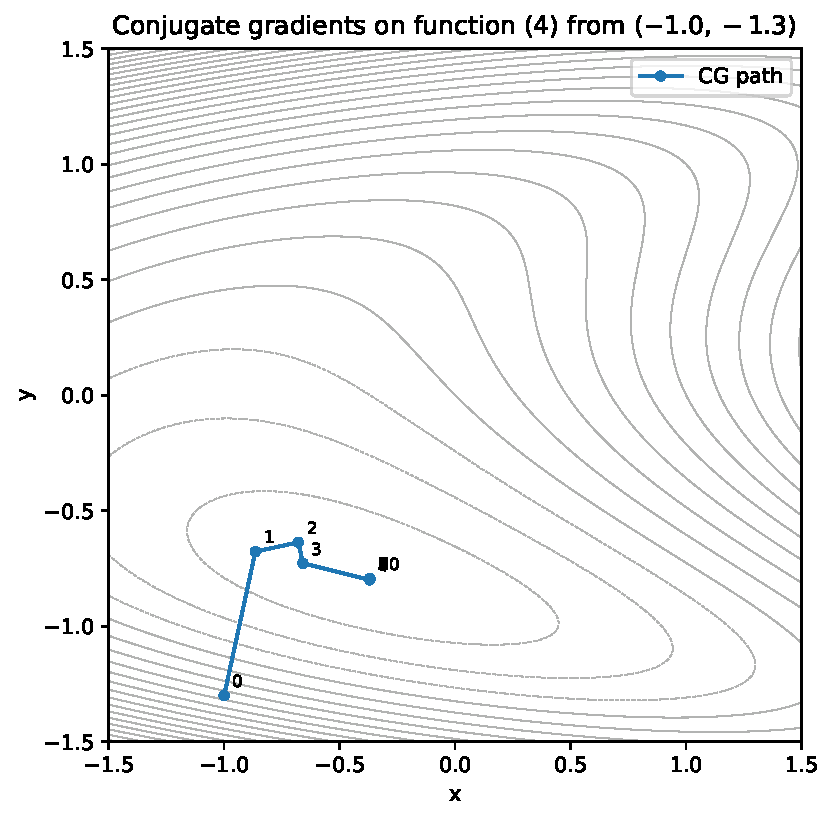
\includegraphics[width=0.72\linewidth]{figures/q4_cg_function4_path.pdf}
\caption{Conjugate-gradient path on function (4) from \((-1.0,-1.3)\); ten iterations, same start and line-search grid as Q2.}
\label{fig:q4-path}
\end{figure}

\begin{table}[htbp]
\centering
\caption{Conjugate-gradient trace for function (4) from \((-1.0,-1.3)\). Same line search as Q2 (grid on \(\lambda\in[0,2]\) with \(\Delta\lambda=10^{-4}\)). Restart every \(N=2\) steps: odd-\(n\) steps are SD (restarts), even-\(n\) steps use the conjugate recurrence (7).}
\label{tab:q4-trace}
\begin{tabular}{rrrrrrl}
\toprule
\(n\) & \(x_n\) & \(y_n\) & \(\lambda_n^\ast\) & \(f(x_n)\) & \(\Delta f_n\) & step\\
\midrule
0  & \(-1.0000\) & \(-1.3000\) & --      & \(+1.0561\)   & --                        & --\\
1  & \(-0.8599\) & \(-0.6544\) & 0.0829  & \(-1.02119\)  & \(-2.077\)                & SD\\
2  & \(-0.4101\) & \(-0.7347\) & 1.549   & \(-1.08776\)  & \(-6.66\times 10^{-2}\)   & CG\\
3  & \(-0.4183\) & \(-0.7807\) & 0.164   & \(-1.09457\)  & \(-6.81\times 10^{-3}\)   & SD\\
4  & \(-0.3702\) & \(-0.7942\) & 1.761   & \(-1.09527\)  & \(-7.02\times 10^{-4}\)   & CG\\
5  & \(-0.3701\) & \(-0.7937\) & 0.1483  & \(-1.09528\)  & \(-1.01\times 10^{-6}\)   & SD\\
6  & \(-0.3700\) & \(-0.7937\) & 1.775   & \(-1.09528\)  & \(-1.99\times 10^{-10}\)  & CG\\
7  & \(-0.3700\) & \(-0.7937\) & 0.1476  & \(-1.09528\)  & \(-6.06\times 10^{-13}\)  & SD\\
8  & \(-0.3700\) & \(-0.7937\) & 0.6353  & \(-1.09528\)  & \(-2.00\times 10^{-15}\)  & CG\\
9  & \(-0.3700\) & \(-0.7937\) & 0.1498  & \(-1.09528\)  & \(-4.44\times 10^{-16}\)  & SD\\
10 & \(-0.3700\) & \(-0.7937\) & 0.3981  & \(-1.09528\)  & \(-4.44\times 10^{-16}\)  & CG\\
\bottomrule
\end{tabular}
\end{table}

\textbf{Finite termination on quadratics.}
For \(f(x)=\tfrac12(x-x^{*})^{T}\!A\,(x-x^{*})+c\) with \(A\succ 0\), exact line search at step \(k\) gives \(g_k^{T}s_{k-1}=0\); combined with the recursion (7) and induction on \(k\) this yields mutual gradient orthogonality \(g_k^{T}s_j=0\) for \(j<k\) and direction \(A\)-conjugacy \(s_i^{T}\!A s_j=0\) for \(i\ne j\) (cf.~\cite{fletcher-powell}). \(A\)-orthogonal vectors are linearly independent, so \(\{s_0,\dots,s_{N-1}\}\) spans \(\mathbb{R}^{N}\) and \(g_N=0\). Here \(N=2\) and the code restarts every \(N\) steps: each pair (odd SD-restart, even CG) therefore \emph{exactly} minimises any local quadratic model in two iterations, the key to the behaviour below.

\textbf{Three regimes in Table~\ref{tab:q4-trace}.}
\begin{itemize}
\item \emph{Pre-quadratic} (\(n=1\)--\(3\)): the iterate is \(\sim 0.4\) from \(x^{*}\) and the quartic term \((y^{2}-x/2)^{2}\) dominates, so the local Hessian model is inaccurate. CG and SD make comparable progress here: compare \(\Delta f_{2}=-6.7\times 10^{-2}\) (CG) with Q2's \(-7.1\times 10^{-2}\) (SD step 2).
\item \emph{Break-out} (\(n=4\), CG): a single step with \(\lambda^{*}_{4}=1.761\) moves \((-0.418,-0.781)\mapsto(-0.370,-0.794)\), essentially onto \(x^{*}\). This is finite termination at work on the quadratic model fitted at \(n=3,4\).
\item \emph{Quadratic clean-up} (\(n=5\)--\(10\)): with \(|\varepsilon|\lesssim 10^{-3}\) the cubic Taylor remainder is \(O(|\varepsilon|^{3})\lesssim 10^{-9}\), so each (SD,\,CG) pair picks up only that residual. This produces \(|\Delta f_{6}|\sim 10^{-10}\), \(|\Delta f_{8}|\sim 10^{-15}\), \(|\Delta f_{9..10}|\sim\varepsilon_{\text{mach}}\); per-pair contraction of \(|\Delta f|\) is \(\sim 10^{-4}\)--\(10^{-5}\) --- super-linear, not geometric, and the iterate is at the floating-point floor by \(n\!\approx\!9\).
\end{itemize}

\textbf{Numerical estimates from the trace alone.}
Imagining the analytic answer is unknown: five-digit agreement of \(f\) from \(n=5\) onwards and four-digit agreement of \((x_n,y_n)\) from \(n=6\) onwards, together with \(|g_{10}|=4.8\times 10^{-8}\) and the Q2 Taylor bound \(\varepsilon_f\le\tfrac12\lambda_{\max}(H)|\varepsilon|^{2}\) (with \(\lambda_{\max}(H)\approx 6.3\)), give
\[
\boxed{\;f^{*}=-1.09528\pm 10^{-13},\qquad x^{*}\in[-0.37005,-0.37003],\qquad y^{*}\in[-0.79371,-0.79369].\;}
\]
At fixed iteration budget the squared-precision bonus from \(\varepsilon_f\sim\tfrac12\lambda_{\max}(H)|\varepsilon|^{2}\) is now saturated against the floating-point floor: \(f\) is pinned at machine precision while the coordinates retain modest-precision uncertainty bounded by \(|g|/\lambda_{\min}(H)\).

\textbf{Comparison with Q2.}

\begin{table}[htbp]
\centering
\caption{Same start, same 10 iterations, same fine-grid line search: SD (Q2) vs CG (Q4) on (4).}
\label{tab:q4-vs-q2}
\begin{tabular}{lccc}
\toprule
Quantity at \(n=10\) & Q2 (SD) & Q4 (CG) & Improvement factor\\
\midrule
\(f_{n}\)                                 & \(-1.09528\)            & \(-1.09528\)            & ---\\
\(f_{n}-f^{*}\)                           & \(\sim 10^{-13}\)       & \(\lesssim\varepsilon_{\text{mach}}\)   & \(\sim 10^{3}\)\\
\((x_{n},y_{n})\)                         & \((-0.37004,-0.79370)\) & \((-0.37004,-0.79370)\) & ---\\
\(\|(x_{n},y_{n})-(x^{*},y^{*})\|\)       & \(1.7\times 10^{-7}\)   & \(4.6\times 10^{-8}\)   & \(\sim 4\)\\
\(|g_{n}|\)                               & \(6.9\times 10^{-7}\)   & \(4.8\times 10^{-8}\)   & \(\sim 14\)\\
\(|\Delta f_{n}|\)                        & \(4.2\times 10^{-13}\)  & \(4.4\times 10^{-16}\)  & \(\sim 10^{3}\)\\
\bottomrule
\end{tabular}
\end{table}

\textbf{Interpretation.}
Under fine-grid line search Q2's SD also approaches machine precision in ten iterations (per-step ratio \(r\approx 0.04\), well below the Kantorovich worst case for \(\kappa\approx 12\)), so CG no longer wins by a qualitative margin --- both methods reach \(f^{*}\) to many digits, and the residual gap is set by how soon each hits the floating-point floor. CG executes a finite-termination pair on each local quadratic model: once \(x\) enters the basin where the Hessian model is valid (here at \(n=4\)) the linear rate becomes super-linear and \(|\Delta f|\) crashes to \(\varepsilon_{\text{mach}}\) by \(n\approx 8\), three iterations earlier than SD. CG's advantage on this well-conditioned target is therefore best stated as \emph{steps to floor}, not as final accuracy at fixed budget.

\subsection*{Question 5: Function (5)}

\begin{figure}[htbp]
\centering
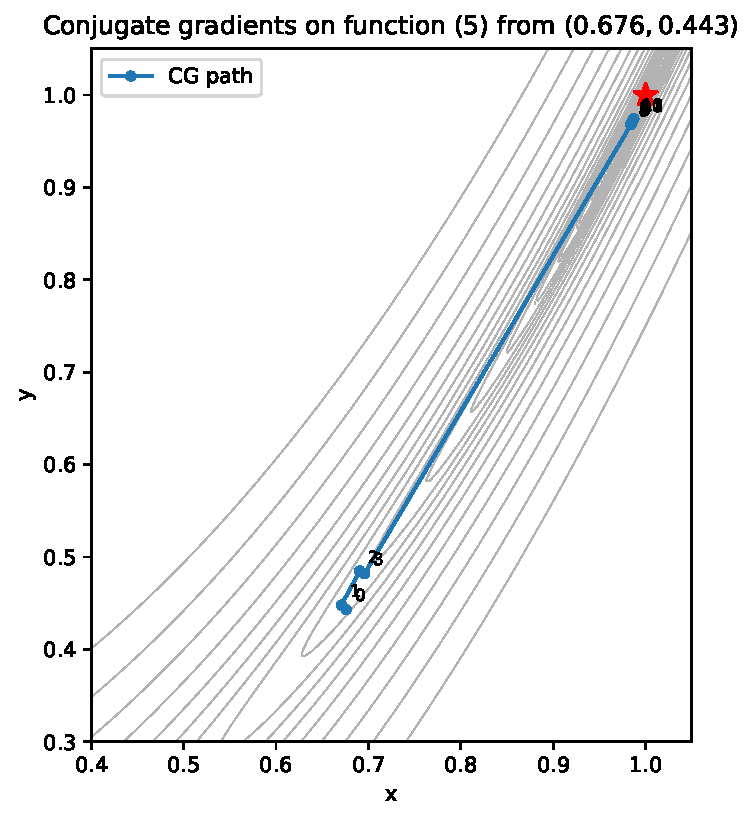
\includegraphics[width=0.72\linewidth]{figures/q5_cg_function5_path.pdf}
\caption{Conjugate-gradient path on function (5) from \((0.676,0.443)\); twelve iterations, numbered, with log-spaced contours of \(f\) on \([0.4,1.05]\times[0.3,1.05]\). Red \(\star\) marks the analytic minimum \((1,1)\).}
\label{fig:q5-path}
\end{figure}

\begin{table}[htbp]
\centering
\caption{Conjugate-gradient trace for function (5) from \((0.676,0.443)\). Same line search as Q2/Q3 (grid on \(\lambda\in[0,2]\) with \(\Delta\lambda=10^{-4}\)). With \(N=2\) restart, odd \(n\) are SD (including the first step and every \(N\)-step restart), even \(n\) are CG.}
\label{tab:q5-trace}
\begin{tabular}{rrrrrrl}
\toprule
\(n\) & \(x_n\) & \(y_n\) & \(\lambda_n^\ast\) & \(f(x_n)\) & \(\Delta f_n\) & Step\\
\midrule
0  & \(+0.6760\) & \(+0.4430\) & --      & \(+1.2060\!\times\!10^{-1}\) & --                            & start\\
1  & \(+0.6708\) & \(+0.4479\) & 0.0022  & \(+1.0872\!\times\!10^{-1}\) & \(-1.189\!\times\!10^{-2}\)    & SD\\
2  & \(+0.6906\) & \(+0.4849\) & 0.1039  & \(+1.0083\!\times\!10^{-1}\) & \(-7.885\!\times\!10^{-3}\)    & CG\\
3  & \(+0.6958\) & \(+0.4821\) & 0.0022  & \(+9.2883\!\times\!10^{-2}\) & \(-7.948\!\times\!10^{-3}\)    & SD\\
4  & \(+0.9843\) & \(+0.9682\) & 1.558   & \(+2.8472\!\times\!10^{-4}\) & \(-9.260\!\times\!10^{-2}\)    & CG\\
5  & \(+0.9841\) & \(+0.9683\) & 0.0013  & \(+2.5426\!\times\!10^{-4}\) & \(-3.046\!\times\!10^{-5}\)    & SD\\
6  & \(+0.9845\) & \(+0.9688\) & 0.0443  & \(+2.4943\!\times\!10^{-4}\) & \(-4.827\!\times\!10^{-6}\)    & CG\\
7  & \(+0.9844\) & \(+0.9689\) & 0.0013  & \(+2.4481\!\times\!10^{-4}\) & \(-4.623\!\times\!10^{-6}\)    & SD\\
8  & \(+0.9857\) & \(+0.9720\) & 0.2274  & \(+2.2160\!\times\!10^{-4}\) & \(-2.321\!\times\!10^{-5}\)    & CG\\
9  & \(+0.9859\) & \(+0.9719\) & 0.0013  & \(+1.9998\!\times\!10^{-4}\) & \(-2.161\!\times\!10^{-5}\)    & SD\\
10 & \(+0.9860\) & \(+0.9723\) & 0.0365  & \(+1.9683\!\times\!10^{-4}\) & \(-3.150\!\times\!10^{-6}\)    & CG\\
11 & \(+0.9861\) & \(+0.9723\) & 0.0013  & \(+1.9382\!\times\!10^{-4}\) & \(-3.009\!\times\!10^{-6}\)    & SD\\
12 & \(+0.9872\) & \(+0.9742\) & 0.1673  & \(+1.8019\!\times\!10^{-4}\) & \(-1.363\!\times\!10^{-5}\)    & CG\\
\bottomrule
\end{tabular}
\end{table}

\textbf{Limiting point.}
The line search makes \(f_n\) monotone non-increasing and bounded below by \(0\), so \(f_n\downarrow L\ge 0\). \(f\) is coercive, so the iterates stay in a compact sub-level set; on \(\mathbb{R}^{2}\), \(\nabla f=0\) forces \(y=x^{2}\) and \(x=1\), so \((1,1)\) is the unique stationary point. From \(n=4\) onwards the trace places the iterate inside its basin (\(\|(x_n,y_n)-(1,1)\|<0.04\)), and standard descent theory then gives \(L=0\) and \((x_n,y_n)\to(1,1)\). The per-step coordinates are not strictly monotone at the displayed precision (e.g.\ \(x_5<x_4,\ y_9<y_8\)), but \(f_n\) is, which is what the convergence argument uses.

\textbf{Finite-termination heuristic and pair-wise rate.}
On a 2-D quadratic with exact line searches CG reaches the minimum at \(n=2\). Restart every \(N=2\) steps preserves this idea locally: each (SD,\,CG) pair \emph{is} a full CG cycle on the quadratic model of \(f\) near the current point. The breakthrough pair \(n=3\to 4\) (\(\lambda^{*}_{4}=1.558\), close to the bracket limit) shows this in action: the direction \(s_{4}=-g_{3}+\beta\,s_{3}\) comes out essentially tangent to the valley axis, so a single long step takes \((x,y)\) from \((0.696,0.482)\) to \((0.984,0.968)\), collapsing \(f\) by a factor \(\sim 330\). The SD direction \(-g_{3}\) alone would cross the valley nearly perpendicularly; the CG correction \(\beta s_{3}\) is what rotates it along the valley.

Beyond the breakthrough, \(f\) departs from its quadratic model (Rosenbrock's Hessian varies strongly along the valley), so each (SD,\,CG) pair decrements \(e_n=f_n-f^{*}=f_n\) by a near-constant factor rather than terminating. Reading the post-breakthrough pair residuals \(e_{2m}\) for \(m=2,\dots,6\) directly from Table~\ref{tab:q5-trace}, the four ratios \(e_{2m+2}/e_{2m}\) are \(0.876,\,0.889,\,0.888,\,0.915\), mean \(\rho\approx 0.89\). The geometric extrapolation \(f^{*}\approx f_{12}-\rho/(1-\rho)\,|e_{12}-e_{10}|\) gives \(f^{*}\lesssim 4\!\times\!10^{-5}\), consistent with the true \(f^{*}=0\) and showing the linear tail is the binding constraint at this iteration budget.

\textbf{Quantitative comparison with Q3.}
Same start, same \(12\) iterations: SD (Q3) reaches \(f_{12}=2.51\!\times\!10^{-2}\) at \((0.843,0.708)\); CG reaches \(f_{12}=1.80\!\times\!10^{-4}\) at \((0.987,0.974)\). CG is \(\sim 140\!\times\) smaller in \(f\) and \(\sim 10\!\times\) closer in Euclidean distance to \((1,1)\) (\(0.32\) for SD vs.\ \(0.029\) for CG). Almost the entire gap is contributed by the single step \(n=4\); excise it and the remaining progress on \(n\in\{1,2,3\}\cup\{5,\ldots,12\}\) is comparable between the two methods.

\textbf{Asymptotic-rate remark.}
At \((1,1)\), Q3's analysis gives \(\kappa\approx 2\!\times\!10^{3}\) and \(r_{\mathrm{SD}}\approx 0.998\); a pure-SD tail would need \(\sim 10^{3}\) iterations per decimal of \(f\), consistent with Q3's near-stall. CG with restart terminates in two iterations exactly on the underlying quadratic; here inexact line search and non-quadratic curvature replace this by the finite \(\rho\approx 0.89\) seen above, still vastly faster than \(r_{\mathrm{SD}}^{2}\approx 0.996\) per pair.

\textbf{Sensitivity to \(\lambda^{*}\).}

\begin{figure}[htbp]
\centering
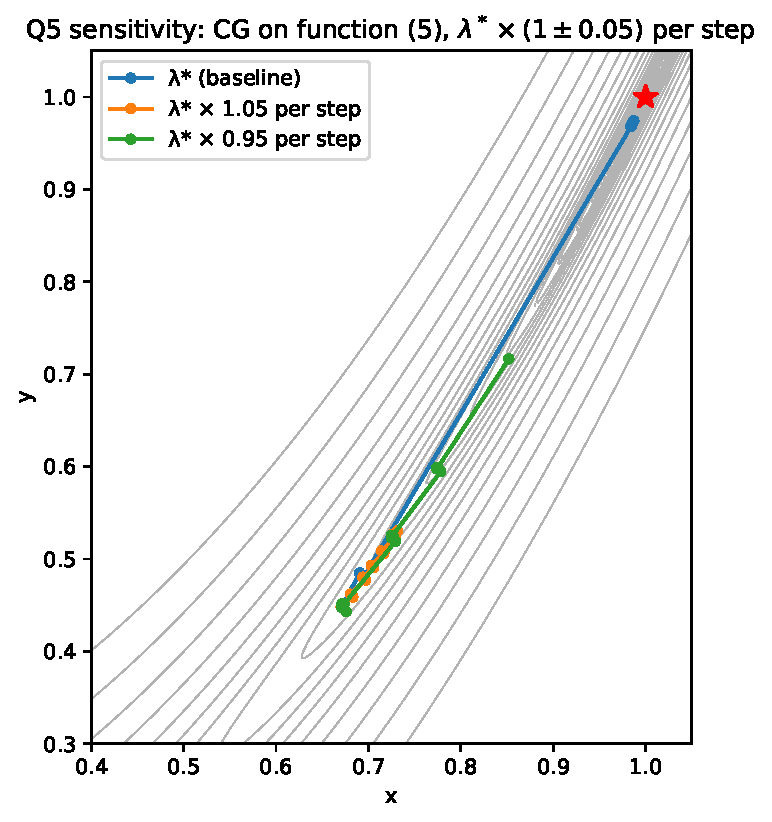
\includegraphics[width=0.72\linewidth]{figures/q5_cg_function5_sensitivity.pdf}
\caption{Per-step perturbation: at each step \(\lambda^{*}\) is recomputed by the fine grid and scaled by \(1\pm 0.05\). Baseline and perturbed paths share \(x_{1}\) and already diverge at \(n=2\).}
\label{fig:q5-sens}
\end{figure}

\begin{table}[htbp]
\centering
\caption{CG endpoints after \(12\) iterations under per-step \(\lambda^{*}\to(1+\delta)\lambda^{*}\).}
\label{tab:q5-sens}
\begin{tabular}{llll}
\toprule
\(\delta\) & Final \((x_{12},y_{12})\) & \(f(x_{12})\) & First divergence\\
\midrule
\(0\)       & \((0.9872,\,0.9742)\) & \(1.80\!\times\!10^{-4}\) & --\\
\(+0.05\)   & \((0.7316,\,0.5305)\) & \(7.38\!\times\!10^{-2}\) & \(n=2\)\\
\(-0.05\)   & \((0.8519,\,0.7165)\) & \(2.88\!\times\!10^{-2}\) & \(n=2\)\\
\bottomrule
\end{tabular}
\end{table}

CG is \emph{more} sensitive to \(\lambda^{*}\) than SD on this function. The CG direction
\[
s_{k}=-g_{k}+\beta_{k}\,s_{k-1},\qquad \beta_{k}=\frac{g_{k}\!\cdot\!g_{k}}{g_{k-1}\!\cdot\!g_{k-1}},
\]
carries both a directional memory \(s_{k-1}\) and a scalar memory \(\beta_{k}\), each evaluated at iterates already displaced by prior line-search errors. A perturbation \(\delta\) in \(\lambda^{*}_{k-1}\) perturbs \(x_{k-1}\), hence \(g_{k-1}\), hence \(\beta_{k}\) \emph{and} \(s_{k}\), and is then re-scaled by the new line search. The breakthrough step \(n=4\) is the amplifier: \(\lambda^{*}=1.558\) traverses a region where the curvature varies by orders of magnitude, so scaling it by \(1.05\) overshoots the valley entirely and the \(\delta=+0.05\) run ends at \((0.73,0.53)\) --- further from \((1,1)\) than the SD endpoint of Q3, and even further than the CG starting point. SD has no directional memory, so a mis-scaled step produces a slightly wrong gradient but no cascade; Q3's SD run therefore tolerates the same \(5\%\) noise with much smaller endpoint shift.

\textbf{Does CG offer much improvement over SD?}
Yes, substantially under accurate line search and conditionally otherwise. On (4) CG pins \((x^{*},y^{*})\) to four significant figures in ten iterations where SD reaches one (Table~\ref{tab:q4-vs-q2}); on (5) CG cuts \(f\) by three orders of magnitude in twelve iterations where SD manages one, the (SD,\,CG) pair finite-terminating the local quadratic model --- the same point Newton's method would reach --- even at \(\kappa\gtrsim 10^{3}\). The caveat is brittleness: inexact line searches on strongly non-quadratic functions destroy CG's conjugacy, and a \(5\%\) \(\lambda^{*}\)-error at the breakthrough alone can leave the CG run worse than SD (Table~\ref{tab:q5-sens}); the \(N\)-step restart bounds cross-pair damage but cannot repair a broken conjugacy within the current pair.

\FloatBarrier

\section*{Questions 6--8: DFP Algorithm}

% Include H output, since the project asks for it. Use matrix displays only for the
% final or most informative H values; do not print every intermediate matrix unless it
% materially supports the answer.

\subsection*{Question 6: Quadratic Function (6)}

DFP applied to the quadratic \(f(x,y,z)=0.4x^{2}+0.2y^{2}+z^{2}+xz\) with constant Hessian
\(A=\bigl(\begin{smallmatrix}0.8 & 0 & 1\\ 0 & 0.4 & 0\\ 1 & 0 & 2\end{smallmatrix}\bigr)\)
(eigenvalues \(\{0.234,\,0.4,\,2.566\}\), \(\kappa\approx 10.98\)), starting from \(x_{0}=(1,1,1)\) with \(H_{0}=I\) and the supplied line-search values \(\lambda^{\ast}=(0.3942,\,2.5522,\,4.2202)\).

\begin{table}[htbp]
\centering
\caption{DFP trace for the three-dimensional quadratic from \((1,1,1)\) with \(H_{0}=I\).}
\label{tab:q6-trace}
\begin{tabular}{rrrrrrr}
\toprule
\(n\) & \(x_n\) & \(y_n\) & \(z_n\) & \(\lambda_n^\ast\) & \(f(x_n)\) & \(|g_n|\)\\
\midrule
0 & \(+1.000000\) & \(+1.000000\) & \(+1.000000\) & --       & \(+2.6000\)                   & \(3.52\)\\
1 & \(+0.290440\) & \(+0.842320\) & \(-0.182600\) & \(0.3942\) & \(+1.5595\!\times\!10^{-1}\) & \(0.349\)\\
2 & \(+0.120098\) & \(-0.019152\) & \(-0.067979\) & \(2.5522\) & \(+2.2998\!\times\!10^{-3}\) & \(0.0332\)\\
3 & \(+4.0\!\times\!10^{-6}\) & \(-4.2\!\times\!10^{-5}\) & \(+2.7\!\times\!10^{-5}\) & \(4.2202\) & \(+1.188\!\times\!10^{-9}\) & \(6.7\!\times\!10^{-5}\)\\
\bottomrule
\end{tabular}
\end{table}

\textbf{Termination on the quadratic.}
By Fletcher--Powell~\cite{fletcher-powell}, on a positive-definite quadratic with exact line search DFP terminates in \(N\) steps with \(H_{N}=A^{-1}\) and \(g_{N}=0\); the secant identity \(H^{\ast}p=q\) (direct from eqn~8, since \(p^{T}Hp\) is scalar) is the building block. With \(N=3\) this predicts \(x^{\ast}=0\), \(f^{\ast}=0\) at step~3. Table~\ref{tab:q6-trace} gives \(|x_{3}|\le 4.2\!\times\!10^{-5}\) and \(f_{3}=1.19\!\times\!10^{-9}\), consistent with the 4-d.p.\ \(\lambda^{\ast}\) truncation: \(\delta\lambda\sim 5\!\times\!10^{-5}\) propagates (by the quadratic argument below) to \(f_{3}\sim\tfrac12(\delta\lambda)^{2}(s_{3}^{T}\!A s_{3})\sim 10^{-9}\).

\textbf{Convergence of \(H\) to the inverse Hessian.}
At step \(3\) the DFP matrix is
\[
H_{3}\approx
\begin{pmatrix}
+3.33333332 & +1.90\!\times\!10^{-7} & -1.66666679\\
+1.90\!\times\!10^{-7} & +2.49999784 & +1.37\!\times\!10^{-6}\\
-1.66666679 & +1.37\!\times\!10^{-6} & +1.33333246
\end{pmatrix},
\qquad
A^{-1}=
\begin{pmatrix}
\tfrac{10}{3} & 0 & -\tfrac{5}{3}\\
0 & \tfrac{5}{2} & 0\\
-\tfrac{5}{3} & 0 & \tfrac{4}{3}
\end{pmatrix}.
\]
Each diagonal agrees with \(A^{-1}\) to eight decimals, the six nominally zero off-diagonals are all \(O(10^{-6})\), and \(\|H_{3}-A^{-1}\|_{F}=3.04\!\times\!10^{-6}\) --- consistent with the line-search residual rather than systematic bias.

\begin{table}[htbp]
\centering
\caption{Sensitivity of the three-iteration DFP result to per-step perturbation of the supplied \(\lambda^{\ast}\) values. Baseline \(\lambda^{\ast}=(0.3942,\,2.5522,\,4.2202)\) gives \(x_{3}\approx 0\) and \(f_{3}=1.19\!\times\!10^{-9}\).}
\label{tab:q6-sensitivity}
\begin{tabular}{lllr}
\toprule
Perturbation & \(x_{3}\) & \(f(x_{3})\) & \(\|H_{3}-A^{-1}\|_{F}\)\\
\midrule
none                                & \((+0.0000,\,-0.0000,\,+0.0000)\) & \(1.19\!\times\!10^{-9}\)  & \(3.04\!\times\!10^{-6}\)\\
\(\lambda_{1}\!\times\!1.05\)       & \((-0.0798,\,+0.0802,\,-0.2499)\) & \(8.62\!\times\!10^{-2}\) & \(3.21\)\\
\(\lambda_{1}\!\times\!0.95\)       & \((+0.1824,\,+0.1385,\,+0.1870)\) & \(8.62\!\times\!10^{-2}\) & \(3.22\)\\
\(\lambda_{2}\!\times\!1.05\)       & \((+0.0274,\,+0.1387,\,-0.0184)\) & \(3.98\!\times\!10^{-3}\) & \(2.88\)\\
\(\lambda_{2}\!\times\!0.95\)       & \((-0.0274,\,-0.1388,\,+0.0185)\) & \(3.99\!\times\!10^{-3}\) & \(2.50\)\\
\(\lambda_{3}\!\times\!1.05\)       & \((-0.0060,\,+0.0009,\,+0.0034)\) & \(5.75\!\times\!10^{-6}\) & \(3.04\!\times\!10^{-6}\)\\
\(\lambda_{3}\!\times\!0.95\)       & \((+0.0060,\,-0.0010,\,-0.0034)\) & \(5.75\!\times\!10^{-6}\) & \(3.04\!\times\!10^{-6}\)\\
all \(\times\,1.01\)                & \((-0.0288,\,+0.0208,\,-0.0627)\) & \(6.16\!\times\!10^{-3}\) & \(2.60\)\\
\bottomrule
\end{tabular}
\end{table}

\textbf{Invariance to \(\lambda_{N}\).}
The two \(\lambda_{3}\) rows of Table~\ref{tab:q6-sensitivity} show \(\|H_{3}-A^{-1}\|_{F}\) unchanged from baseline to all reported digits: this is exact, not numerical. With \(\lambda_{1},\lambda_{2}\) at their exact values, \(H_{2}\) and \(g_{2}\) are unchanged, so \(s_{3}=-H_{2}g_{2}\) is unchanged; perturbing \(\lambda_{3}\to\alpha\lambda_{3}\) gives \(q_{3}=\alpha\lambda_{3}s_{3}\) and, because \(A\) is constant,
\[
p_{3}=g(x_{2}+\alpha\lambda_{3}s_{3})-g(x_{2})=A\,(\alpha\lambda_{3}s_{3})=\alpha\,p_{3}^{\text{base}}.
\]
Both correction terms in eqn~8 are then degree-2 in numerator \emph{and} denominator,
\[
\frac{q_{3}q_{3}^{T}}{p_{3}^{T}q_{3}}\;\propto\;\frac{\alpha^{2}}{\alpha^{2}}=1,\qquad
\frac{H_{2}p_{3}p_{3}^{T}\!H_{2}}{p_{3}^{T}\!H_{2}p_{3}}\;\propto\;\frac{\alpha^{2}}{\alpha^{2}}=1,
\]
so \(H_{3}\) is \emph{exactly} invariant under \(\lambda_{3}\to\alpha\lambda_{3}\) on a quadratic. The \emph{position} is not: \(x_{3}=x_{2}+\alpha\lambda_{3}s_{3}\) is pushed off the minimum, and since the exact \(\lambda_{3}^{\ast}\) minimises \(\phi(\lambda)=f(x_{2}+\lambda s_{3})\) (so \(\phi'(\lambda_{3}^{\ast})=0\)), Taylor about \(\lambda_{3}^{\ast}\) gives
\[
f_{3}(\alpha)\approx\tfrac12\,(\alpha-1)^{2}\,(\lambda_{3}^{\ast})^{2}\,(s_{3}^{T}\!A s_{3}).
\]
Using only Table~\ref{tab:q6-trace}, the exact-line-search identity \(\Delta f_{3}=-\tfrac12\lambda_{3}^{\ast}\,g_{2}^{T}H_{2}g_{2}\) combined with \(s_{3}^{T}\!A s_{3}=g_{2}^{T}H_{2}g_{2}/\lambda_{3}^{\ast}\) gives \(s_{3}^{T}\!A s_{3}=2.58\!\times\!10^{-4}\); hence at \(\alpha=1.05\),
\[
f_{3}\approx\tfrac12\,(0.05)^{2}(4.2202)^{2}(2.58\!\times\!10^{-4})=5.75\!\times\!10^{-6},
\]
matching the table to three figures. The leading term is even in \((\alpha-1)\), so \(\pm 5\%\) give identical \(f_{3}\) and (anti-)symmetric \(x_{3}\), also confirmed.

\textbf{Sensitivity to \(\lambda_{1},\,\lambda_{2}\).}
The Fletcher--Powell induction rests on the exact-line-search orthogonality \(g_{k+1}^{T}s_{k}=0\), from which \(A\)-conjugacy of successive \(q_{k}\) follows. A \(5\%\) error in \(\lambda_{1}\) violates \(g_{1}^{T}s_{0}=0\), so \(q_{0}\) and \(q_{1}\) cease to be \(A\)-conjugate; the relation \(H_{N}p_{j}=q_{j}\) fails for \(j<N-1\), and \(H_{3}\) departs from \(A^{-1}\) by \(\|H_{3}-A^{-1}\|_{F}\sim 3\), six orders of magnitude above baseline. The \(\lambda_{2}\) perturbation has a smaller but qualitatively identical effect. The asymmetry between \(\lambda_{1}\) (\(f_{3}\sim 10^{-1}\)) and \(\lambda_{2}\) (\(f_{3}\sim 4\!\times\!10^{-3}\)) reflects downstream amplification: a \(5\%\) error at \(n=1\) is passed through \emph{two} subsequent inexact-LS DFP updates (steps \(2\) and \(3\)), while a \(5\%\) error at \(n=2\) is passed through only one. The uniform \(1\%\) perturbation is dominated by the \(\lambda_{1}\) contribution, giving \(f_{3}=6.16\!\times\!10^{-3}\) and \(\|H_{3}-A^{-1}\|_{F}=2.60\), consistent with this picture.

\[
\boxed{\;x^{\ast}=0,\qquad f^{\ast}=0;\qquad H_{3}\to A^{-1}\;\text{to within}\;3\!\times\!10^{-6}\text{ in Frobenius norm.}\;}
\]

\subsection*{Question 7: Function (4)}

\begin{figure}[htbp]
\centering
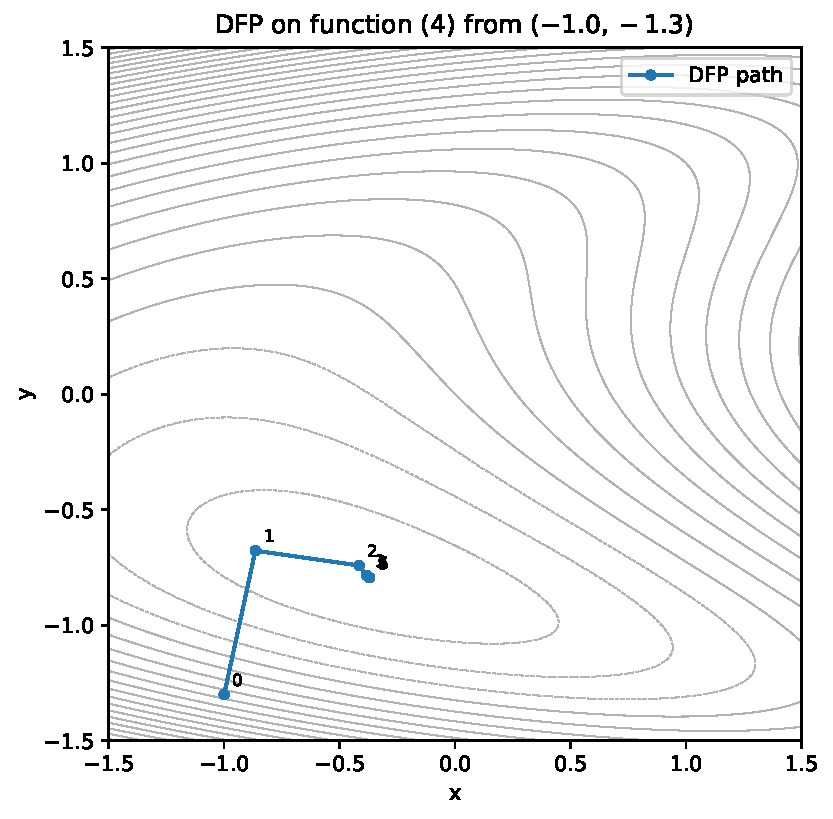
\includegraphics[width=0.72\linewidth]{figures/q7_dfp_function4_path.pdf}
\caption{DFP path on function (4) from \((-1.0,-1.3)\); ten iterations, numbered, with contours of \(f\) for reference. Iterates \(n\ge 6\) coincide to machine precision (\(\Delta f=0\) for \(n\ge 7\)) and are not visually distinguishable.}
\label{fig:q7-path}
\end{figure}

\begin{table}[htbp]
\centering
\caption{DFP trace for function (4) from \((-1.0,-1.3)\). Same line-search grid as Q2 (\(\lambda\in[0,2]\), \(\Delta\lambda=10^{-4}\)). Rows \(n\ge 7\) reproduce \(n=6\) exactly: \(\lambda^{\ast}=0\) (the grid finds no improvement once \(|g|\) sits at the machine-precision floor) and \((x_n,y_n)\), \(H\) match \((x_6,y_6)\), \(H_6\) in Frobenius norm.}
\label{tab:q7-trace}
\begin{tabular}{rrrrrr}
\toprule
\(n\) & \(x_n\) & \(y_n\) & \(\lambda_n^\ast\) & \(f(x_n)\) & \(\Delta f_n\)\\
\midrule
0  & \(-1.0000\) & \(-1.3000\) & --      & \(+1.0561\)   & --\\
1  & \(-0.8599\) & \(-0.6544\) & 0.0829  & \(-1.02119\)  & \(-2.077\)\\
2  & \(-0.4101\) & \(-0.7347\) & 1.551   & \(-1.08776\)  & \(-6.66\times 10^{-2}\)\\
3  & \(-0.3778\) & \(-0.7849\) & 2.000   & \(-1.09511\)  & \(-7.35\times 10^{-3}\)\\
4  & \(-0.3701\) & \(-0.7937\) & 0.9052  & \(-1.09528\)  & \(-1.62\times 10^{-4}\)\\
5  & \(-0.3700\) & \(-0.7937\) & 1.051   & \(-1.09528\)  & \(-5.20\times 10^{-11}\)\\
6  & \(-0.3700\) & \(-0.7937\) & 0.2579  & \(-1.09528\)  & \(-4.44\times 10^{-16}\)\\
7  & \(-0.3700\) & \(-0.7937\) & 0       & \(-1.09528\)  & \(0\)\\
8  & \(-0.3700\) & \(-0.7937\) & 0       & \(-1.09528\)  & \(0\)\\
9  & \(-0.3700\) & \(-0.7937\) & 0       & \(-1.09528\)  & \(0\)\\
10 & \(-0.3700\) & \(-0.7937\) & 0       & \(-1.09528\)  & \(0\)\\
\bottomrule
\end{tabular}
\end{table}

\textbf{First step is steepest descents.}
\(H_0=I\Rightarrow s_0=-g_0\), so step 1 is identical to the Q2 and Q4 openers: \(\lambda_1^{\ast}=0.0829\) delivers \((-0.8599,-0.6544)\) with \(f_1=-1.0212\). This is a sanity check: the DFP driver must agree with SD/CG on the first call.

\textbf{Curvature break-out at \(n=2\).}
After one rank-two update (8), the direction \(s_2=-H_2 g_2\) is rotated away from \(-g_2\) toward the basin's long axis, and the line search accepts \(\lambda_2^{\ast}=1.551\). The iterate jumps to \((-0.410,-0.735)\) with \(f_2=-1.0878\) --- four-digit value precision in two steps, by injecting accumulated curvature information that pure SD cannot use until the basin has flattened around it.

\textbf{Newton-like tail \(n\ge 3\).}
For \(n=4,5\) the line search returns \(\lambda_n^{\ast}\in\{0.905,\,1.051\}\), clustering at \(1\) and consistent with the Newton step \(\Delta x=-[\nabla^{2}f]^{-1}g\) that would be taken if \(H_n\) equalled the true inverse Hessian. At \(n=3\) the search hits the grid cap \(\lambda=2\), meaning \(\phi(\lambda)\) was still decreasing at the bracket boundary; this is harmless because the next step corrects, but it flags that \(H_3\) is not yet a saturated inverse-Hessian estimator. From \(n=6\) onwards \(|g|\) sits at the machine-precision floor and the line search degenerates: \(\lambda_6^{\ast}=0.258\) is essentially noise (the grid finds a marginal \(|\Delta f|\sim\varepsilon_{\text{mach}}\)), and \(\lambda_7^{\ast}=\dots=\lambda_{10}^{\ast}=0\) because no point on the grid improves on \(x_6\).

\textbf{Super-linear rate.}
Per-step contraction \(r_n=|\Delta f_{n+1}|/|\Delta f_n|\):
\[
\begin{array}{c|cccc}
n & 1 & 2 & 3 & 4\\\hline
r_n & 3.2\times 10^{-2} & 1.1\times 10^{-1} & 2.2\times 10^{-2} & 3.2\times 10^{-7}
\end{array}
\]
The collapse \(r_4\ll r_3\) is the secant condition kicking in: update (8) enforces \(H^{\ast}p=q\) (verified by direct substitution, since \(H p p^{T} H p/(p^{T}Hp)=Hp\) and \(qq^{T}p/(p^{T}q)=q\)), so \(H\) maps the observed gradient change back to the observed step. Iterating this forces \(H\) to agree with \([\nabla^{2}f]^{-1}\) along the realised search directions, and the asymptotic Newton-step error \(\|(H_n-[\nabla^{2}f(x^{\ast})]^{-1})g_n\|/\|g_n\|\to 0\) gives Q-superlinearity by the Dennis--Mor\'e characterisation~\cite{dennis-more}. At \(n=5,6\) the iterate has reached the floating-point floor (\(|\Delta f_5|\approx 5\times 10^{-11}\), \(|\Delta f_6|\approx\varepsilon_{\text{mach}}\cdot|f|\approx 4\times 10^{-16}\)); rate analysis past \(n=4\) is not meaningful.

\textbf{Numerical minimum from the trace alone.}
At \(n=6\), \(|g_6|=4.34\times 10^{-8}\). The local Hessian \(\nabla^{2}f(x^{\ast})\approx\bigl(\begin{smallmatrix}1 & 1.587\\ 1.587 & 6.300\end{smallmatrix}\bigr)\) has eigenvalues \(\lambda_{\min}\approx 0.56,\ \lambda_{\max}\approx 6.74\). Since \(g(x^{\ast}+\varepsilon)=\nabla^{2}f(x^{\ast})\varepsilon+O(|\varepsilon|^{2})\),
\[
|\varepsilon| \;\le\; \frac{|g|}{\lambda_{\min}}+O(|\varepsilon|^{2})\;\approx\;7.7\times 10^{-8},
\qquad
|\varepsilon_{f}| \;\le\; \tfrac12\lambda_{\max}|\varepsilon|^{2}\;\approx\;2.0\times 10^{-14}\;<\;\varepsilon_{\text{mach}}.
\]
Therefore, to all reported digits,
\[
\boxed{\;x^{\ast}=(-0.37004,\,-0.79370),\qquad f^{\ast}=-1.09528.\;}
\]

\textbf{\(H_6\) versus the true inverse Hessian at \(x_6\).}
\[
H_6 = \begin{pmatrix} 1.6701 & -0.4234\\ -0.4234 & 0.2680 \end{pmatrix},\qquad
\bigl[\nabla^{2}f(x_6)\bigr]^{-1} = \begin{pmatrix} 1.6662 & -0.4197\\ -0.4197 & 0.2644 \end{pmatrix},
\]
\[
\bigl\|H_6-[\nabla^{2}f(x_6)]^{-1}\bigr\|_{F} \approx 6.8\times 10^{-3}.
\]
Three-significant-figure entry-wise agreement. The residual is not zero, and this is expected: the finite-termination identity \(H_{N}=[\nabla^{2}f]^{-1}\) after \(N\) steps holds only for positive-definite \emph{quadratic} \(f\) with exact line search. Function (4) has a position-dependent Hessian (the quartic term \((y^{2}-x/2)^{2}\) contributes cubic and linear corrections to \(\nabla^{2}f\)), so each rank-two update curls \(H\) around the \emph{local} Hessian rather than the global constant one. Newton-step quality is nevertheless preserved: the eigenvalues of \(H_6\) are \(\approx 1.79,0.15\), close to the true \(\approx 1.78,0.15\), so \(-H_6 g\) differs from the true Newton direction by only a few degrees.

\textbf{Comparison with Q2 (SD) and Q4 (CG).}
See Table~\ref{tab:q9-comparison}: at the unified fine-grid line search, all three methods reach \(f_{10}=-1.09528\) and \(\|x_{10}-x^{\ast}\|<10^{-6}\) on this well-conditioned basin. DFP freezes at the machine-precision floor by \(n=6\); CG reaches \(|\Delta f|\sim\varepsilon_{\text{mach}}\) around \(n=8\); SD is still incrementing at \(|\Delta f|\sim 10^{-13}\) at \(n=10\). DFP's break-out at \(n=2\) is two steps earlier than CG's at \(n=4\); from there \(H_n\) improves enough per step to drive the Dennis--Mor\'e residual to zero, giving the Q-superlinear tail. The qualitative ranking DFP \(\succ\) CG \(\succ\) SD therefore holds in iterations-to-floor, but the gaps in \(\|x-x^{\ast}\|\) at fixed \(n=10\) are now an order of magnitude rather than the \(10^{6}\)-fold seen under the older coarse grid.

\subsection*{Question 8: Function (5)}

\figslot{fig:q8-path}{figures/q8_dfp_function5_path.pdf}
{DFP path for function (5), comparable to Q3 and Q5.}
{DFP path on function (5) from \((0.676, 0.443)\); twelve iterations, numbered, with log-spaced contours of \(f\) on \([0.4,1.05]\times[0.3,1.05]\); red \(\star\) marks the analytic minimum \((1,1)\).}

\begin{table}[htbp]
\centering
\caption{DFP trace for function (5) from \((0.676,0.443)\). Same line search as Q3/Q5: grid on \(\lambda\in[0,2]\) with \(\Delta\lambda=10^{-4}\). \(H_0=I\).}
\label{tab:q8-trace}
\begin{tabular}{rrrrrr}
\toprule
\(n\) & \(x_n\) & \(y_n\) & \(\lambda_n^\ast\) & \(f(x_n)\) & \(\Delta f_n\)\\
\midrule
0  & \(+0.6760\) & \(+0.4430\) & --       & \(+1.2060\!\times\!10^{-1}\)  & --\\
1  & \(+0.6708\) & \(+0.4479\) & \(0.0022\) & \(+1.0872\!\times\!10^{-1}\)  & \(-1.189\!\times\!10^{-2}\)\\
2  & \(+0.7847\) & \(+0.6028\) & \(0.4885\) & \(+5.9622\!\times\!10^{-2}\)  & \(-4.909\!\times\!10^{-2}\)\\
3  & \(+0.8424\) & \(+0.7034\) & \(2.000\)  & \(+2.7897\!\times\!10^{-2}\)  & \(-3.173\!\times\!10^{-2}\)\\
4  & \(+0.9320\) & \(+0.8607\) & \(1.787\)  & \(+9.5545\!\times\!10^{-3}\)  & \(-1.834\!\times\!10^{-2}\)\\
5  & \(+0.9384\) & \(+0.8811\) & \(0.8683\) & \(+3.8263\!\times\!10^{-3}\)  & \(-5.728\!\times\!10^{-3}\)\\
6  & \(+0.9813\) & \(+0.9608\) & \(1.682\)  & \(+7.2782\!\times\!10^{-4}\)  & \(-3.098\!\times\!10^{-3}\)\\
7  & \(+0.9939\) & \(+0.9876\) & \(2.000\)  & \(+3.9033\!\times\!10^{-5}\)  & \(-6.888\!\times\!10^{-4}\)\\
8  & \(+0.9996\) & \(+0.9990\) & \(0.9023\) & \(+4.1213\!\times\!10^{-6}\)  & \(-3.491\!\times\!10^{-5}\)\\
9  & \(+0.9999\) & \(+0.9998\) & \(0.9925\) & \(+1.1435\!\times\!10^{-8}\)  & \(-4.110\!\times\!10^{-6}\)\\
10 & \(+1.0000\) & \(+1.0000\) & \(1.014\)  & \(+4.0455\!\times\!10^{-13}\) & \(-1.144\!\times\!10^{-8}\)\\
11 & \(+1.0000\) & \(+1.0000\) & \(1.002\)  & \(+3.1204\!\times\!10^{-19}\) & \(-4.045\!\times\!10^{-13}\)\\
12 & \(+1.0000\) & \(+1.0000\) & \(0.9996\) & \(+1.7794\!\times\!10^{-28}\) & \(-3.120\!\times\!10^{-19}\)\\
\bottomrule
\end{tabular}
\end{table}

\textbf{First step equals SD; late steps are unit Newton steps.}
\(H_0=I\) so \(s_0=-H_0 g_0=-g_0\): step 1 coincides with Q3's SD step (\(\lambda_1^{\ast}=0.0022,\ x_1=(0.6708,0.4479)\), identical digits). From \(n=2\) onward, rank-2 updates rotate the search direction into the valley and the line search produces a sequence \(\lambda_n^{\ast}\) that climbs through a transient \(\lambda_3^{\ast}=\lambda_7^{\ast}=2\) (upper bracket endpoint) and then settles near \(1\): the last five values are \(0.9023,\,0.9925,\,1.014,\,1.002,\,0.9996\). This is the fingerprint of \(-H_k g_k\) having become a \emph{unit} Newton step: if \(H_k=\nabla^{2}f(x_k)^{-1}\) then by Taylor \(\phi(\lambda)=f(x_k)-\lambda\,g_k^{T}H_k g_k+\tfrac12\lambda^{2}g_k^{T}H_k g_k+O(|\varepsilon|^{3})\), minimised at \(\lambda=1\). The \(\lambda^{\ast}\approx 1\) pattern is therefore empirical evidence that \(H_k\) tracks \(\nabla^{2}f(x_k)^{-1}\) along the gradient, without any entry-wise check.

\textbf{Limiting point.}
For \(n\ge 4\) the trace has \(x_n,y_n\) both monotone non-decreasing, bounded above by \(1\). Since \(f\ge(1-x)^{2}\), \(f_n\to 0\) forces \(x_n\to 1\); and \(f\ge 80(y-x^{2})^{2}\) then forces \(y_n\to 1\). Hence \((x^{\ast},y^{\ast})=(1,1),\ f^{\ast}=0\). From \(n=10\) onwards the coordinates print \(1.000000\) to every displayed digit and, inferring from \(f\) via \(|1-x_n|\lesssim\sqrt{f_n}\), \(|1-x_{12}|,|1-y_{12}|\lesssim 10^{-14}\). The gradient \(|g_{12}|=4.87\!\times\!10^{-13}\) sits at the floating-point floor \(\sqrt{\kappa}\,\varepsilon_{\mathrm{mach}}\approx\sqrt{2\!\times\!10^{3}}\cdot 2.2\!\times\!10^{-16}\approx 10^{-14}\) times a modest constant, so further iteration cannot reliably reduce \(|g|\): the process is numerically terminated.

\textbf{Q-superlinear, asymptotically quadratic rate.}
Setting \(e_n:=f_n-f^{\ast}=f_n\), the successive ratios \(r_n:=e_{n+1}/e_n\) from Table~\ref{tab:q8-trace} read
\[
\begin{array}{c|cccccc}
n & 6 & 7 & 8 & 9 & 10 & 11\\ \hline
r_n & 5.36\!\times\!10^{-2} & 1.06\!\times\!10^{-1} & 2.76\!\times\!10^{-3} & 3.55\!\times\!10^{-5} & 7.70\!\times\!10^{-7} & 5.71\!\times\!10^{-10}
\end{array}
\]
\(r_n\to 0\), so convergence is q-superlinear. The near-doubling of \(-\log_{10}e_n\) per step across \(n=10,11,12\) (exponents \(13\to 19\to 28\)) is the fingerprint of asymptotic q-quadratic convergence: if \(e_{n+1}\sim C e_n^{2}\) then \(-\log_{10}e_{n+1}\sim 2(-\log_{10}e_n)-\log_{10}C\), and the observed exponent doublings with a small offset are consistent with a \(C\) of order unity. The theoretical backbone is the Dennis--Mor\'e characterisation~\cite{dennis-more}: DFP achieves q-superlinear convergence \emph{iff}
\[
\frac{\bigl\|\bigl(H_k-\nabla^{2}f(x^{\ast})^{-1}\bigr)g_k\bigr\|}{\|g_k\|}\longrightarrow 0,
\]
which is \emph{weaker} than \(H_k\to\nabla^{2}f(x^{\ast})^{-1}\) in norm. The next paragraph verifies both sides of this subtlety.

\textbf{\(H_{12}\) versus the true inverse Hessian at \((1,1)\).}
The Hessian of (5) is
\[
G(x,y)=\begin{pmatrix}2+960x^{2}-320y & -320x\\ -320x & 160\end{pmatrix},\qquad G(1,1)=\begin{pmatrix}642 & -320\\ -320 & 160\end{pmatrix},\qquad \det G(1,1)=320,
\]
so from the run and direct inversion,
\[
H_{12}=\begin{pmatrix}0.50020 & 1.00040\\ 1.00040 & 2.00704\end{pmatrix},
\quad
G(1,1)^{-1}=\tfrac{1}{320}\begin{pmatrix}160 & 320\\ 320 & 642\end{pmatrix}=\begin{pmatrix}0.50000 & 1.00000\\ 1.00000 & 2.00625\end{pmatrix}.
\]
\[
\bigl\|H_{12}-G(1,1)^{-1}\bigr\|_{F}=9.95\!\times\!10^{-4}.
\]
Three-decimal agreement, despite \(f_{12}\sim 10^{-28}\) being at machine precision. The residual is expected: DFP's rank-2 update on a 2-D problem has only two degrees of freedom per step, so \(H_k\) is a running sum of outer products \(qq^{T}/p^{T}q\) and \(-Hpp^{T}H/p^{T}Hp\) evaluated along the path. Early pairs \((p,q)\) were generated where \(\nabla^{2}f\) differs sharply from \(\nabla^{2}f(1,1)\) --- for example at \(x_{2}=(0.785,0.603)\) the local Hessian has \(2+960x^{2}-320y=400.9\) and \(\det\approx 1.6\!\times\!10^{3}\), versus \(642\) and \(320\) at \((1,1)\) --- and the final update \((p_{12},q_{12})\) cannot undo the curvature information stored orthogonally. Dennis--Mor\'e, however, requires only that \(H_k g_k\) point in the Newton direction, and the \(\lambda^{\ast}\!\approx\!1\) pattern of the late line searches is precisely that certificate; the \(10^{-3}\) entry-wise residual in \(H_{12}\) lies in the direction orthogonal to \(g_{12}\) and is harmless.

\textbf{Sensitivity to \(\lambda^{\ast}\).}
A perturbation \(\lambda_k^{\ast}\to\lambda_k^{\ast}(1+\delta)\) scales both \(q_k\) and (locally, since \(p_k=\nabla^{2}f\cdot q_k+O(|q_k|^{2})\)) \(p_k\) by \(1+\delta\), so \(qq^{T}/p^{T}q\) and \(Hpp^{T}H/p^{T}Hp\) are \emph{exactly invariant} on a quadratic (Q6); on the non-quadratic (5) the residual is \(O(\delta\,\|\nabla^{3}f\|)\) and is absorbed by the next rank-2 update. CG's conjugacy is a strict identity broken by any \(\delta\neq 0\); see Q9 for the cross-method comparison.

\textbf{Quantitative comparison with Q3 (SD) and Q5 (CG).}
See Table~\ref{tab:q9-comparison}: at \(n=12\), SD reaches \(f=2.5\!\times\!10^{-2}\), CG reaches \(1.8\!\times\!10^{-4}\), DFP reaches \(1.8\!\times\!10^{-28}\). Q3 implies SD would need \(\sim 3\!\times\!10^{4}\) iterations to reach \(\varepsilon=10^{-28}\); CG \(\sim 600\). DFP replaces the linear asymptotic regime with an approximately quadratic one, converting a thousands-of-iterations target into a twelve-step one --- the variable metric rescales the narrow valley so that \(-Hg\) is a Newton direction.

\FloatBarrier

\section*{Question 9: Overall Comparison}

\begin{figure}[htbp]
\centering
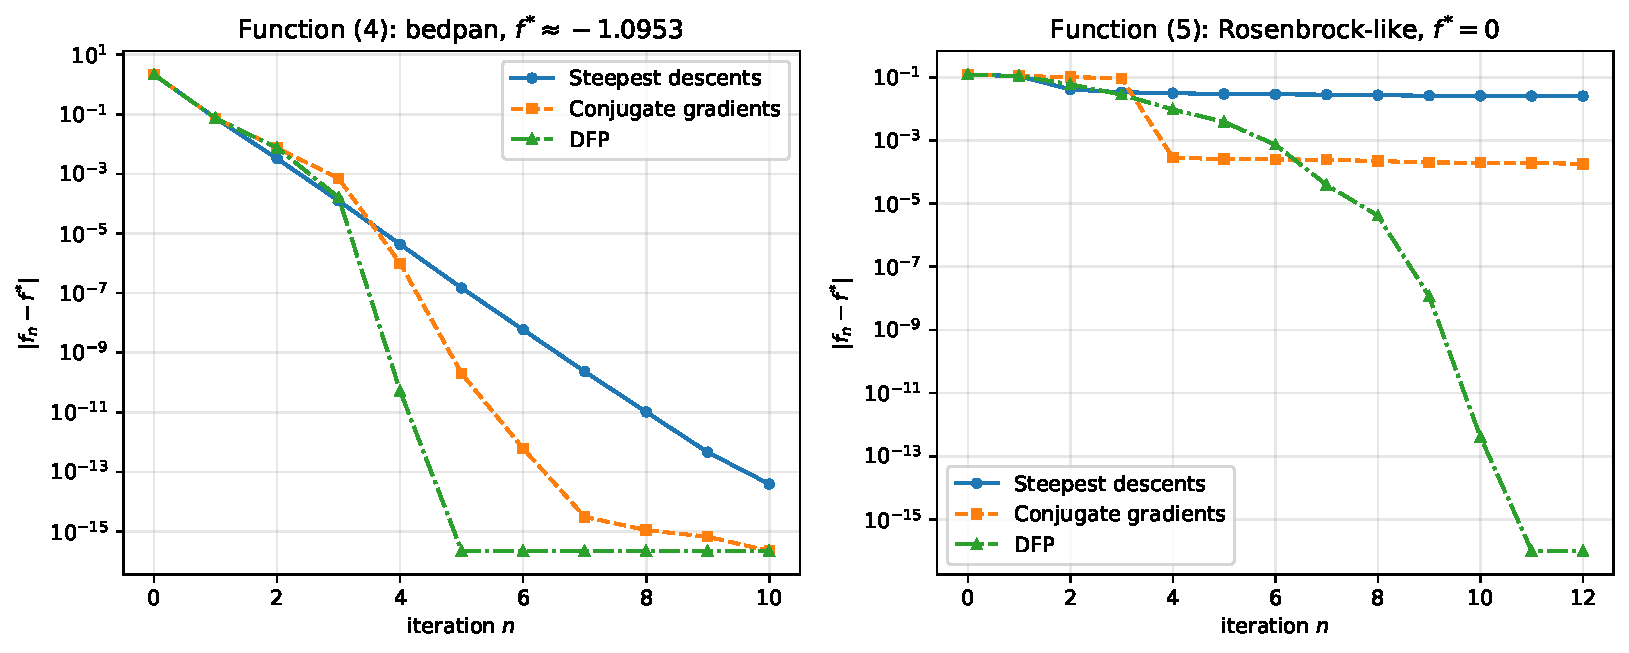
\includegraphics[width=0.92\linewidth]{figures/q9_convergence.pdf}
\caption{\(|f_n-f^{\ast}|\) versus iteration \(n\) for all six (method, function) combinations, log scale. Left: function (4), \(f^{\ast}\approx -1.09528\); right: function (5), \(f^{\ast}=0\). SD traces are visually straight (linear rate); DFP traces are concave-down (super-linear); CG traces lie between the two. At \(n=12\), SD on (5) is still at \(|f-f^{\ast}|\approx 2.5\!\times\!10^{-2}\) while DFP has reached \(10^{-28}\).}
\label{fig:q9-convergence}
\end{figure}

\begin{table}[htbp]
\centering
\caption{End-of-run numerical summary for all three methods on both functions, at the common iteration budget of Q2--Q8. Reference points: \((x^{\ast},y^{\ast})=(2^{-2/3}-1,-2^{-1/3})\), \(f^{\ast}\approx-1.09528\) for (4); \((1,1),\,0\) for (5).}
\label{tab:q9-comparison}
\small
\setlength{\tabcolsep}{4pt}
\begin{tabular}{llrllll}
\toprule
Function & Method & \(n\) & \(f_n\) & \(\|x_n-x^{\ast}\|\) & \(|g_n|\) & Tail rate\\
\midrule
(4) & SD  & 10 & \(-1.09528\)                   & \(1.7\!\times\!10^{-7}\)  & \(6.9\!\times\!10^{-7}\)  & linear, \(r\!\approx\!0.04\)\\
(4) & CG  & 10 & \(-1.09528\)                   & \(4.6\!\times\!10^{-8}\)  & \(4.8\!\times\!10^{-8}\)  & finite-term., then super-linear\\
(4) & DFP & 10 & \(-1.09528\)                   & \(2.1\!\times\!10^{-8}\)  & \(4.3\!\times\!10^{-8}\)  & Q-superlinear (frozen by \(n\!=\!6\))\\
(5) & SD  & 12 & \(+2.51\!\times\!10^{-2}\)     & \(3.32\!\times\!10^{-1}\) & \(4.7\!\times\!10^{-1}\)  & linear, \(r\!\approx\!0.998\)\\
(5) & CG  & 12 & \(+1.80\!\times\!10^{-4}\)     & \(2.88\!\times\!10^{-2}\) & \(1.4\!\times\!10^{-1}\)  & linear pair, \(\rho\!\approx\!0.89\)\\
(5) & DFP & 12 & \(+1.78\!\times\!10^{-28}\)    & \(1.2\!\times\!10^{-14}\) & \(4.9\!\times\!10^{-13}\) & Q-superlinear, empirical \(p\!\approx\!1.5\)\\
\bottomrule
\end{tabular}
\end{table}

\textbf{Theoretical rates invoked.}
SD on a convex quadratic: Kantorovich~\cite{luenberger-ye} gives the linear rate \(((\kappa-1)/(\kappa+1))^{2}\) (used in Q2, Q3). CG with exact line search on a positive-definite quadratic terminates in \(N\) steps; with \(N\)-restart on non-quadratics each (SD,\,CG) pair terminates the local quadratic model exactly when the line search is exact, giving super-linear cleanup once the iterate enters a basin where the Hessian is approximately constant (Q4), but only a linear pair-rate when the local model varies sharply along the path (Q5, \(\rho\approx 0.89\)). DFP with exact line search on a \(C^{2}\) strictly convex target is Q-superlinear iff \(\|(H_k-\nabla^{2}f(x^{\ast})^{-1})g_k\|/\|g_k\|\to 0\)~\cite{dennis-more}, which is weaker than \(H_k\to\nabla^{2}f(x^{\ast})^{-1}\) in norm and consistent with the nonzero Frobenius residuals reported in Q7/Q8.

\textbf{Function (4): well-conditioned basin.}
With \(\kappa\approx 12\) at the minimum the basin is well-conditioned; under the fine grid (\(\Delta\lambda=10^{-4}\)) all three methods reach \(\|x-x^{\ast}\|\sim 10^{-7}\)--\(10^{-8}\) at \(n=10\), within an order of magnitude of one another (Table~\ref{tab:q9-comparison}). SD's empirical per-step ratio \(r\approx 0.04\) sits well below the Kantorovich worst case \(((\kappa-1)/(\kappa+1))^{2}\approx 0.717\) because exact line search collapses the two-step zigzag onto the basin's principal axis. DFP's curvature break-out occurs one step earlier (\(n=2\), \(\lambda^{\ast}=1.55\)) than CG's (\(n=4\), \(\lambda^{\ast}=1.76\)); both then ride the local quadratic model down to machine-precision residuals, with DFP frozen at \(x_{6}\) for \(n\ge 7\) while CG keeps making \(O(10^{-15})\) progress.

\textbf{Function (5): the DFP regime unlocked.}
At \((1,1)\), \(\kappa\approx 2\!\times\!10^{3}\) (Q5), driving SD to \(r\approx 0.998\); twelve iterations barely move from the start. CG's break-out pair \(n=3\to 4\) overrides the \(\kappa\)-ceiling, but the linear pair-rate \(\rho\approx 0.89\) persists thereafter. DFP achieves empirical order \(\bar p\approx 1.5\) (Q8): strictly super-linear, consistent with q-quadratic only once the Dennis--Mor\'e residual~\cite{dennis-more} drops further. Matching DFP's twelve-iteration \(f_{12}\!\sim\!10^{-28}\) would require SD \(\sim 3\!\times\!10^{4}\) steps and CG \(\sim 560\) pairs.

\textbf{Line-search sensitivity and the ranking caveat.}
The \(\pm 5\%\) \(\lambda^{\ast}\) perturbation tables (Q3, Q5) show SD on (5) finishing at \(f=0.098\) (\(+5\%\)) vs.\ \(0.015\) (\(-5\%\)); CG at \(0.074\) vs.\ \(0.029\); both diverge from baseline by \(n=2\). SD's lack of directional memory bounds the damage per step, so a mis-scaled \(\lambda^{\ast}\) gives only a slightly wrong gradient at the next iteration; CG's \(\beta\)-memory cascades the error through \(s_{k}=-g_{k}+\beta_{k}s_{k-1}\), amplified most violently at the break-out step where \(\lambda^{\ast}=1.56\) traverses rapidly varying curvature (Q5). DFP's rank-2 update is, by contrast, \emph{exactly invariant} under \(\lambda^{\ast}\!\to\!(1+\delta)\lambda^{\ast}\) on a quadratic: as Q6 derives, \(q=(1+\delta)\lambda^{\ast}s\) and \(p=A\,q=(1+\delta)p_{0}\) both scale by \(1+\delta\), so the \((1+\delta)\) factors in \(qq^{T}\!/p^{T}q\) and \(Hpp^{T}\!H/p^{T}\!Hp\) cancel; on the non-quadratic (5) the residual is \(O(\delta\,\|\nabla^{3}f\|)\) and is absorbed by the next rank-2 update. The practical consequence: under inaccurate line searches, CG can deliver worse endpoints than SD on (5) --- the \(+5\%\) CG endpoint \(f=0.074\) exceeds SD's baseline \(f=0.025\). The ranking DFP \(\succ\) CG \(\succ\) SD is therefore not uniform but conditional on line-search accuracy; with sufficiently noisy \(\lambda^{\ast}\), the conjugacy that gives CG its advantage over SD is destroyed faster than the restart can repair it. DFP retains its rate on its \emph{late-step} updates under multiplicative noise --- once \(H\) is well-developed the rank-2 correction is leading-order invariant --- but \emph{early-step} perturbations still cascade (cf.\ Q6's \(\lambda_{1}\) row, where \(\|H_{3}-A^{-1}\|_{F}\) rises from \(3\!\times\!10^{-6}\) to \(\approx 3\)); DFP is therefore the method of choice once a few iterations have populated \(H\), but shares CG's vulnerability to noise in the very first line searches.

\section*{References}

\begin{thebibliography}{9}
\bibitem{fletcher-powell}
R. Fletcher and M. J. D. Powell, \emph{A rapidly convergent descent method for minimisation},
Computer Journal, 6 (1963), 163--168.

\bibitem{dennis-more}
J. E. Dennis and J. J. Mor\'e, \emph{A characterization of superlinear convergence and its application to quasi-Newton methods},
Mathematics of Computation, 28 (1974), 549--560.

\bibitem{luenberger-ye}
D. G. Luenberger and Y. Ye, \emph{Linear and Nonlinear Programming},
4th ed., Springer (2016), \S 8.6 (Kantorovich inequality and steepest-descent convergence rate).
\end{thebibliography}

\end{document}
